\documentclass[onehalf,11pt]{beavtex}
\usepackage{algorithmicx}
\usepackage{algpseudocode}
\usepackage{algorithm}
\usepackage{graphicx}
\usepackage{amsmath}
\title{Using RUBI to Partition Agents in Air Traffic Problems with Hard Constraints and Reward Shaping}
\author{William Curran}
\degree{Master of Science}
\doctype{Thesis}
\department{Electrical Engineering and Computer Science}
\depttype{School}
\depthead{Director}
\major{Computer Science}
\advisor{Kagan Tumer}
\submitdate{June 4, 2013}
\commencementyear{2013}

\abstract{Air traffic flow management over the U.S. airpsace is a difficult problem. Current management approaches lead to hundreds of thousands of hours of delay, costing billions of dollars annually. Weather and airport conditions may instigate this delay, but routing decisions balancing delay with congestion contribute significantly to the propagation of delays throughout the US airspace. The task of managing delay may be seen as a multiagent congestion problem. 

In this problem there are many tightly coupled agents whose actions collectively impact the system, making it difficult for agents to learn how they individually affect the system. Reward shaping is effective at improving agent learning for soft constraint problems by reducing noise caused by interactions with other agents, so we extend those results to hard constraints that cannot be easily learned, and must be enforced algorithmically. Additionally, congestion must be removed from the system in order to ensure a safe environment for all aircraft. This can be done through the use of a greedy scheduler, enforcing a ground delay on each plane to remove congestion from the system, at the cost of delay.

Reward shaping reduces noise caused by agent interactions, and a greedy scheduler removes congestion from the system, but these two approaches cannot be simply combined without a large increase in computational complexity. Agent partitioning can be used to alleviate this complexity by treating each partition of agents as an independent set of agents from other partitions, thus simplifying the computation during each learning step.

Our approach is based on the combination of three different methods to perform hard constraint optimization: a greedy scheduler, reward shaping and agent partitioning. We present two agent partitioning algorithms in conjunction with this approach to simplify the learning domain. The first partitioning algorithm uses system features to compute similarities between agents. This is then used to partition agents into small subsets. To remove the assumption of having domain knowledge, we introduce the Reward/Utility Based Impact (RUBI) algorithm. This algorithm develops an effective similarity matrix while requiring no prior domain knowledge. This similarity matrix can then be used in any similarity based partitioning algorithm. Our results show that autonomous partitioning of the agents using system features leads to up to 450x speed over simple hard constraint enforcement, as well as up to a 37\% improvement in performance over a greedy scheduling solution, while using RUBI to partition agents led to a better partitioning of agents, as well as a 510x speed up. Both results correspond to hundreds of hours of delay saved in a single day.}

\acknowledgements{I would like to thank my adviser Dr. Kagan Tumer for always being on my side no matter how many silly mistakes I make (e.g. Submitting an old version of a paper to AAMAS entitled ``Super Awesome Paper'' 1 hour before the deadline) and supporting me both mentally and academically throughout my graduate work. 

I would like to particularly acknowledge Carrie Rebhuhn for proofreading my thesis more times than I (or she) cares to count, for listening to my speech over and over again, for always supporting me in my work, and most importantly, for pacifying our adviser with candy bars before rough meetings. And how could I forget, thank you Carrie Rebhuhn for also introducing me to Boris and Natasha.

And most importantly I would like to acknowledge my mom for her encouragement, support, and patience throughout my last 6 years of college.}


\begin{document}
\maketitle

\mainmatter

\chapter{Introduction}
A primary concern facing the aerospace industry today is the efficient, safe and reliable management of our ever-increasing air traffic. In 2011, weather, routing decisions and airport conditions caused 330,063 delays, accounting for 266,999 hours of delay \cite{faa05}. Many of these delays in the National Airspace System (NAS) are caused by en route, landing, or departing airspace congestion. The number of new flights being scheduled is faster than that of airports being built, making effective traffic control algorithms essential. We refer to the task of managing delay in the system by coordinating aircraft as the Air Traffic Flow Management Problem (ATFMP). 

Typical methods to alleviate delay in the ATFMP involve imposing ground delay on aircraft, changing the speed of en route aircraft, and changing separation between aircraft. Because the airspace has many connections from one airport to another, the congestion and associated delay can propagate throughout the system. Delays may be imposed to better coordinate aircraft and mitigate the propagation of congestion and the associated delay, but which aircraft should be delayed? The search space in such a problem is huge, as there are tens of thousands of flights every day within the United States \cite{faa05}.

Current approaches to the ATFMP include the use of binary integer programming \cite{Bertsimas}, evolutionary approaches \cite{Rios}, and multiagent reinforcement learning \cite{tumer-agogino_jaamas12}. The most recent complete overview of the ATFMP in practice is provided by Sridhar, Grabbe, and Mukherjee \cite{Sridhar}. These approaches reduce delay in the NAS, but either have not been expanded to an entire day of aircraft data or does not completely remove all congestion from the system. 

We propose an approach to solving the problem that blends multiagent coordination, reward shaping, hard constraints, and automated agent partitioning. Multiagent coordination turns the ATFMP into a distributed problem, thus decomposing it into smaller, more manageable problems. This coordination typically improves performance, but makes modeling interactions between agents much more difficult. When an agent takes an action with many other agents, the total reward of the system may not reflect the contribution of the single agent. 

Reward shaping is a field of multiagent reinforcement learning that focuses on the design of rewards, and has been shown to assist in multiagent coordination. The difference reward is a reward shaping technique that is helpful in discovering how much a single agent contributed to the overall system reward by calculating only the portion of the global reward to which a particular agent directly contributed. The combination of multiagent coordination and reward shaping give the ability to perform an intelligent guided search over tens of thousands of aircraft actions, while the hard constraint on congestion ensures a safe airspace.

In the ATFMP, multiagent coordination with reward shaping becomes a computationally intractable task, therefore we used automated agent partitioning to reduce the overhead associated with the hard constraint while computing rewards. Agents were only required to compute the reward relative to other agents within their partition, removing thousands of extra computations per learning step. We first use automated agent partitioning that required domain knowledge and partitioned agents based on predicted agent interactions. To further generalize this work we then implement the Reward/Utility Based Impact (RUBI), a novel automated agent partitioning algorithm using zero prior domain knowledge.

RUBI learns an effective partitioning of agents, while requiring no domain knowledge. It asks the question: What is each agent's local reward with agent $a$ and without agent $a$? The difference in these two rewards is the impact on one agent to agent $a$. We first test RUBI in a simple heterogeneous bar problem as a benchmark, where partitioning with RUBI finds an optimal solution more efficiently than the straight learning approach. We then apply this algorithm to a more difficult problem, the ATFMP, where partitioning with RUBI leads to better quality partitions, leading to faster simulations and better learning.

A high level view of the approach is as follows: First, we compute partitions of agents. These partitions are treated as reward independent of each other, and therefore need to only compute rewards relative to the other agents within their partition. We will use the term \textit{reward independent} to denote one partition of agents to have no impact on the reward of other partitions. Essentially, no matter what actions one partition of agents take, it will not affect the the action choice for any agent in another partition. We then perform multiagent reinforcement learning using the difference reward. Lastly, we introduce a greedy scheduler, removing all congestion from the system at the cost to delay. Again, combining the multiagent reinforcement learning with reward shaping and the greedy scheduler turns this into a computationally intractable task. However, with agent partitioning, rewards can be computed many times faster with minimal performance degradation.

This paper is organized as follows: In Section 2 we will describe our domains, the field of multiagent systems and our related work. This will be the foundation of the rest of the work in this paper. In Section 3 we will then introduce our approach by explaining the agent definition, agent learning, reward function, the heuristic approaches used, and how this all works together as hard constraint optimization, and our simulator. We will then introduce both partitioning methods, domain-based partitioning and partitioning using RUBI. In Section 5 we will first show the results for learning in the ATFMP while using domain-based partitioning, then we will show partitioning with RUBI working in both the heterogeneous bar problem and ATFMP, lastly we will analyze the difference in results between the standard partitioning algorithm and RUBI. We will conclude in Section 6 with a discussion of the results.

The contributions of this thesis are largely based on the blending of multiagent reinforcement learning, the difference reward and hard constraints. We also introduce the Reward/Utility Based Impact algorithm, a partitioning algorithm that removes the need for prior domain knowledge. There are two main contributions to this thesis:

\begin{itemize}
\item We combined multiagent reinforcement learning using the difference reward with hard constraints. Since this is typically a computationally intractable task, the problem required hard constraint optimization through the use of agent partitioning. 

\item We introduce the Reward/Utility Based Impact (RUBI) algorithm, removing any need for domain-specific information while partitioning, and creating well performing partitions with very little effort from the programmer.

\end{itemize}

We show that this partitioning approach leads to a variety of performances, balancing the cost of time complexity and the benefits of improved performance, and allowing a user to choose whether to optimize time complexity or performance. 

We also show that with reward independent partitions, the RUBI algorithm performs no worse than partitioning using domain-based partitioning, but with faster simulations. By computing reward-based impact, reward independent partitions computed with RUBI are smaller than domain-based partitions. When not reward independent, partitions using RUBI outperform partitions using domain-based similarity scores. Since RUBI computes reward-based impact, partitions created using RUBI are created based on how much impact they have on other agents within their partitioning, essentially making partitions smaller, but no less informative. It can also be used to discover non-trivial agent coupling, leading to a better partitioning in domains where the interactions between agents are not obvious. 

\chapter{Background}
In this section we provide background information which is key to understanding the approach used in this paper. Section 2.1 gives the reader a basic understanding of what multiagent learning is, the reward shaping technique used in this thesis, and a brief overview of work in agent coordination and how it is used in reinforcement learning. Section 2.2 explains the classic clustering algorithm used in this paper, Hierarchical Agglomerative Clustering. Section 2.3 is the related work, explaining previous approaches to the Air Traffic Flow Management Problem (ATFMP) and partitioning in complex systems. Lastly, Section 2.4 introduces the domains used in this paper, the heterogeneous bar problem and the ATFMP.

\section{Multiagent Systems}

The field of multiagent systems is the combination of artificial intelligence and distributed problem solving. This section discusses how distributed problem solving is used with learning algorithms from artificial intelligence in order to collectively solve problems. Section 2.1.1 provides background in the reinforcement learning tools used to solve multiagent problems, Section 2.1.2 discusses the current field of multiagent learning and how it is used to solve distributed problems, and the section concludes with background on constraint optimization, and the reasoning behind using our constraint optimization approach over others. Section 2.1.3 explains the reward shaping approach used in this work, and Section 2.1.4 is a breif overview of the work in agent coordination.

\subsection{Reinforcement Learning}

Reinforcement learning is a tool within the field of multiagent or single-agent learning where agents take an action, observe the environment, and receive a reward based on the new environment \cite{Sutton98reinforcementlearning}. Reinforcement learners can learn with and without a model of the environment. In this work we use model-free stateless multiagent reinforcement learning. Without a state transition model, reinforcement learners take actions solely based on previous experience and the current timestep, and have no concept of state. There are three main aspects when defining a stateless reinforcement learner: the mapping, the reward function, and action-value updates.

The mapping is a map from a value to the current optimal action an agent has learned to take. Initially the agents start with an arbitrary mapping, which is iteratively adjusted based on the reward received and the action-value updates.

The reward function encompasses the high-level goal of the system. When an agent takes an action that is good for the system, the reward function ideally returns to the agent a positive reward proportional to how much it helped the system-level reward. Reinforcement learners also ideally receive a correspondingly smaller reward when their actions are detrimental to the system. In this way agents can iteratively update to converge to the optimal policy according to their reward design. This update is based on the action-value updates.

Action-value updates of the agents mapping are based on the reward received. Equation \ref{eq:Action Value Learning Update} show the action-value update \cite{Sutton98reinforcementlearning}: 

\begin{equation} \label{eq:Action Value Learning Update}
V_t(a) \leftarrow V_{t-1}(a) + \alpha (R_t(a) - V_{t-1}(a))\;,
\end{equation}

where $V_t(a)$ is the updated action-value table entry for action $a$, $V_{t-1}(a)$ is the previous action-value table entry for action $a$, $\alpha$ is the learning rate between 0 and 1 (1 causing the agent to only take the most recent reward into account and 0 causing no update), and $R_t$ represents the reward received this time step for taking action $a$. In a static environment, if the $\alpha$ term is chosen too high the agent will have a hard time finding the best long term policy, and if it is set too low an agent will take a long time to reach the optimal policy. In a constantly changing environment $\alpha$ needs to be set to a rate close to the rate of change. If set too low the environment will change faster than the agent is learning the environment, and if set too high the same problems arise as in the static environment \cite{Sutton98reinforcementlearning}.

In action-value learning agents enforce $\epsilon$-greedy action selection, where the best policy is chosen with probability $1 - \epsilon$ and a random policy with probability $\epsilon$. The Algorithm \ref{alg:Action Value Learning Algorithm} explains the typical formulation of action-value learning:

\begin{algorithm} \label{alg:Action Value Learning Algorithm}
  \caption{Action-Value Learning}
  \begin{algorithmic}[1]
    \Statex
    \Function{Action-Value Learner}{}
      \State{Initialize V arbitrarily}     
	  \For{$e \leftarrow 1$ to $Episodes$}
	  \State{$s \leftarrow initialize$}
	    \For{$t \leftarrow 1$ to $Timesteps$}      
          \State{$a \leftarrow argmax_a V_t(a)$ with probability $1 - \epsilon$ otherwise $a \leftarrow$ random}
          \State{Take action a, observe $r$ and $s'$}
          \State{$V_t(a) \leftarrow V_{t-1}(a) + \alpha (r - V_{t-1}(a))$}
          \State{$s \leftarrow s'$}
        \EndFor
      \EndFor
     \EndFunction
  \end{algorithmic}
\end{algorithm}


\subsection{Multiagent Learning}

Multiagent learning is the intersection between the fields of multiagent systems and machine learning. Typical machine learning tasks include classification, function approximation, and problem solving, where multiagent systems deals with distributed problem solving in domains involving many agents interacting. Distributed problem solving decomposes the tasks into smaller, more manageable problems allowing individual agents to collectively solve the problem. The multiagent system approach leads to a solution that is scaleable and more robust to unmodeled system dynamics, but modeling agent interactions are typically complicated. Multiagent learning works toward solving this problem by allowing an agent to learn interactions required to improve the performance of their team \cite{tuyls2006learning}.

In our multiagent system we have many reinforcement learners learning in parallel. Agents take an action simultaneously, and receive feedback based on the system state after those actions have been simulated. When performing reinforcement learning for a single agent the concept of receiving a reward based on an action is simple, but in a multiagent system many problems arise, namely the credit assignment problem.

In multiagent reinforcement learning, the credit assignment problem is the task of distributing a reward signal to agents that accurately represents their impact on the system level reward. A domain with many agents as well as highly-coupled actions suffers when using the system-level or local rewards. System-level rewards allow an agent to identify whether the joint action of all the agents increases the system's performance, but cannot determine whether its own action produces the increase or if another agent was responsible. This leads to a noisy reward signal. Local rewards can always identify whether an action had some positive or negative effects, but these local rewards do not allow agents to coordinate effectively. In highly-coupled domains local rewards hurt system-level performance, while the high number of agents cause agents to learn slowly from system-level rewards due to the noise. In addition, these system-level rewards tend to converge to suboptimal policies. Reward shaping is a typical solution to this problem.

\subsection{Reward Shaping for Coordination}

Multiagent coordination is an important aspect of many domains, such as data routing \cite{tumer-wolpert_jair02}, air traffic control \cite{tumer-agogino_jaamas12, Sislak:2008:AMA:1402744.1402755}, Robocup soccer \cite{AAMAS12-agmon}, rover coordination \cite{5509316} and power plant operations \cite{Colby:2012:SFF:2343576.2343637}. A learning or evolutionary algorithm will often convert a once computationally intractable search problem into a feasible guided search. 

In learning algorithms reward design is important in keeping convergence time low while keeping performance high. In many multiagent coordination domains there is a difference between maximizing the system-level reward and maximizing a single agent's reward. If an agent always takes the locally-optimal action, it does not always maximize the system-level reward; this is known as the Tragedy of the Commons \cite{Hardin}.

The difference reward \cite{tumer-wolpert_jair02} is evaluated such that each agent's reward is related to the individual's contribution to team performance, therefore the signal-to-noise ratio is improved considerably. This leads to final better policies at an accelerated convergence rate, as well as overcoming the Tragedy of the Commons. The difference reward is defined as:

\begin{equation}
D_i(z) = G(z) - G(z - z_i + c_i)\;,
\end{equation}

where \textit{z} is the system state, $z_i$ is the system state with agent $i$, and $c_i$ is a counterfactual replacing agent $i$. This counterfactual offsets the artificial impact of removing an agent from the system. For example, removing an aircraft from the system always artificially decreases the amount of congestion and delay, which would provide a poor reward if a counterfactual is not used.

The difference reward provides a compact encapsulation of the agent's impact on the system. It reduces the noise from other agents in the reward signal and has outperformed both system-level and local rewards in many congestion domains \cite{AAMAS12-agmon, tumer-agogino_jaamas08, Agogino:2012:ELS:2330163.2330306, Colby:2012:SFF:2343576.2343637, Sislak:2008:AMA:1402744.1402755, tumer-wolpert_jair02}. In many systems it is difficult or impossible to calculate the difference reward without resimulation, which can become prohibitively costly. If resimulation is fast, or the difference reward function is easily approximated, this reward function is a powerful tool for multiagent coordination.

\subsection{Agent Coordination}

Agent coordination \cite{Nwana96co-ordinationin} is another approach to reduce the noise of other agents found in multiagent learning. There are three main approaches to reducing this noise: hierarchical methods, task-based decomposition and team formation. Hierarchical methods and task-based decomposition are typically performed as a preliminary step to simplify the learning domain, while team formation is often performed online. 

Hierarchical methods decompose large problems into smaller ones, overcomes partial observability, and re-uses subtasks. This organizational structure leads to many benefits, such as faster learning and learning from fewer trials. Haizheng Zhang and Victor Lesser \cite{Zhang-406} used hierarchical methods to develop a hierarchical agent group formation protocol as an alternative to a flat peer-to-peer organizational sharing system, demonstrating a significant increase in performance. On a more theoretical application, MAXQ by Dietterich et. al \cite{Dietterich00hierarchicalreinforcement} decomposes a Markov Decision Process (MDP) into a hierarchy of smaller MDPs and decomposes the value function of the target MDP into an additive combination of the value functions of the smaller MDPs. Our work similarly decomposes a large task into many semi-independent smaller tasks, essentially simultaneously solving many smaller, and therefore easier problems.

Similar to hierarchical methods, task-based decomposition decomposes large problems into many smaller, more task-specific problems. Agents are grouped together in teams that are specialized for a specific task. An agent can explore more parts of the state relevant to its current task rather than exploring the entire state space, and therefore learn faster \cite{Doucette:2012:HTD:2330163.2330178, 4708962}. Task-based decomposition has been previously applied in robotics for cellular manufacturing \cite{399902}, where the complexity of the manufacturing process is too large for a straightforward multiagent approach, and the authors use task-based decomposition.  Task-based decomposition has also been used in pattern recognition \cite{788664} to simplify image classification through the use of decomposing pattern classification problems based on the task required.

In team formation, agents only learn with respect to other agents within the same team. Team formation is traditionally the problem of selecting the best possible team to accomplish a certain goal, given limited resources. Typically, certain skills are necessary to accomplish a task, and we must select a team that has all the necessary skills with the minimum cost \cite{Guttmann_makingallocations, Guestrin:2002:CRL:645531.757784}. Team formation has been in rover coordination \cite{Knudson:2010:RCA:1838206.1838422}, search and rescue in disaster response \cite{Guestrin:2002:CRL:645531.757784, Tambe97towardsflexible}, and many other domains.

Similar to the work of Dietterich et. al, we use hierarchical methods to decompose a larger learning problem into a series of smaller and easier to solve problems. This allows agents to ignore much of the state space and find a good policy at a much faster rate. The reasoning behind the need to do this is explained in Section 3.

\section{Agent Partitioning}

Clustering is the task of grouping a set of objects in such a way that objects within a group are more similar to each other than to other groups. In this work, the objects being clustered are agents. When clustering is applied to agents, it is known as agent partitioning. This section will discuss the  different types of machine learning clustering algorithms and our reasoning behind choosing Hierarchical Agglomerative Clustering.

\subsection{Clustering algorithms}

The two most common and basic forms of clustering are centroid-based clustering and connectivity based clustering. Both are have costs and benefits. Here we analyze those costs and benefits and explain which we use in this work.  

In centroid-based clustering, clusters are represented by a central vector, which may not necessarily be a member of the data set. K-means clustering is a common approach when the object can be represented by features. In k-means clustering, the number of clusters are fixed to k, leading to an intuitive optimization problem: find the cluster centers and assign the objects to the nearest cluster center, such that the squared distances from the cluster are minimized. K-means clustering is a commonly employed clustering technique and has been used in hundreds of applications over the years \cite{Jain:2010:DCY:1755267.1755654}.

Connectivity based clustering, also known as hierarchical clustering, is based on the core idea of objects being more related to nearby objects than to objects farther away. In this method of clustering, typically an $n$x$n$ similarity matrix is computed, where $n$ is the number of objects to cluster. After the similarity matrix is computed, this hierarchical clustering can be performed, clustering objects one at a time based on the similarity matrix, until one cluster remains. Clustering can be stopped at any point and saved to obtain a varying number of clusters. Like k-means clustering, hierarchical clustering has been used in hundreds of applications for many years, including document clustering \cite{Zhao:2002:EHC:584792.584877} and drug design \cite{Bottegoni15072006}.

In this work, we choose not to use centroid-based clustering. In centroid-based clustering, a feature vector must be created for every agent. In domains with tens of thousands of agents, such as air traffic, this becomes a very large memory requirement. We chose to use a form of hierarchical clustering, hierarchical agglomerative clustering. The work in this thesis is focused around developing a similarity matrix that can be used as input to the hierarchical agglomerative clustering algorithm.

\subsection{Hierarchical Agglomerative Clustering}
 
The HAC algorithm first computes an $N$ x $N$ similarity matrix $C$ and an $N$-sized indicator matrix $I$ where $N$ is the number of agents. Each element is initially considered to be in its own cluster. The algorithm then executes $N$-1 iterations of clustering, starting with the most similar clusters according to the similarity matrix. In each iteration two clusters are merged together, the similarity matrix is updated based on the newly merged cluster and every other cluster, and the indicator matrix for that cluster is set to 0. $SIM(d_n, d_i)$ and $SIM(i,m,j)$ are functions computing the similarity between clusters, where $SIM(d_n, d_i)$ is the initial similarity between $d_n$ and $d_i$, and $SIM(i,m,j)$ is the similarity between merged clusters $i$ and $m$, and another cluster $j$.

There are currently three main methods of computing cluster similarity $SIM(i,m,j)$: 1. Single-link, where the updated similarity between the merged cluster and other clusters is the minimum distance $i$ or $m$ has to $j$. 2. Complete-link, where the updated similarity between the merged cluster and other clusters is the maximum distance $i$ or $m$ has to $j$. 3. Average-link, where the updated similarity between the merged cluster and other clusters is the average distance $i$ and $m$ has to $j$. In this work we use the average-link similarity in order to try to obtain closely sized clusters.

In this work we chose to seed the initial similarity matrix $C$ with a similarity computed by either using prior domain knowledge, such as flight plan similarity, or using RUBI, thus replacing $SIM(d_n, d_i)$.

%\begin{table}[]
%\begin{tabular}{|c|c|}
%\hline
%Name & Formula\\
%\hline
%Single-Link&$min\{d(a,b) : a \in A, b \in B\}$ \\
%\hline
%Complete-Link&$max\{d(a,b) : a \in A, b \in B\}$ \\
%\hline
%Average-Link & $\frac{1}{|A| |B|} \sum_{a \in A}\sum_{b \in B} d(a,b)$\\
%\hline
%\end{tabular}
%\caption{How $Sim$ is traditionally computed, where $d$ is a distance metric and $A$ and $B$ are the two cluster sets.}
%\label{Linking}
%\end{table}

\begin{algorithm}
  \caption{Hierarchical Agglomerative Clustering}
  \begin{algorithmic}[1]
    \Statex
    \Function{HAC}{$d_1,..., d_N$}
	  \For{$n \leftarrow 1$ to $N$} \hspace{25 mm} (Initialize Similarity Matrix $C$)
	    \For{$i \leftarrow 1$ to $N$}      
          \State{$C[n][i] \leftarrow SIM(d_n, d_i)$}
          \EndFor
          \State{$I[n] \leftarrow 1$ \hspace{37 mm} (keeps track of active clusters)}
        \EndFor
        \State{$A \leftarrow []$}
        \For{$k \leftarrow 1$ to $N-1$} \hspace{20 mm} (assembles clustering as a sequence of merges)
          \State{$<i, m>$ $\leftarrow$ $argmax_{<i,m>: i \neq m \wedge I[i]=1 \wedge I[m]=1}$ C[i][m]} 
          \State{$A.APPEND(<i,m>)$ 	\hspace{10 mm} (store merge)}
          \For{$j \leftarrow 1$ to $N$}
            \State{C[i][j] $\leftarrow SIM(i,m,j)$}
           	\State{C[j][i] $\leftarrow SIM(i,m,j)$}
          \EndFor
          \State{I[m] $\leftarrow$ 0}
        \EndFor
      \State \Return{$A$}
    \EndFunction
  \end{algorithmic}
\end{algorithm}

\section{Related Work}

This section discusses the previous work in the ATFMP, constraint optimization, and agent partitioning. Section 2.3.1 discusses the previous work in the ATFMP, and the specific issues behind what has been previously applied. Section 2.3.2 shows the issues of previous methods and how RUBI and algorithmically enforced hard constraints solve them. Lastly, Section 2.3.3 gives an overview of previously developed agent partitioning algorithms.

\subsection{Air Traffic Flow Management Problem}

Previous work in the ATFMP and scheduling had applied Integer Linear Programming \cite{Bertsimas}, evolutionary approaches \cite{Agogino:2009:EEM:1570256.1570258, Rios}, and multiagent approaches \cite{tumer-agogino_jaamas12,Curran:2013:AHC:2484920.2485183, 664154, Sislak:2008:AMA:1402744.1402755, Zhang95areinforcement}. The ATFMP is a naturally distributed problem with complex interactions among all aircraft and airports. This renders predetermined centralized solutions suboptimal whenever there is any deviation from the expected air traffic flow. Therefore using a decentralized multiagent system is an ideal approach in such a domain.

There are three main issues to using Integer Linear Programming (ILP) that are removed using a multiagent approach; first, designing an ILP algorithm for a particular task is a difficult process, and it takes a lot of effort to adapt ILP to new problem variations that inevitably come up. Second, a formulation of ILP is complex even for simple problems. For real world implementations there is an enormous amount of subtle complexity that has to be included in the system, such as balancing the needs to airlines, air traffic controllers and passengers. These complexities can be added in a straightforward way in reward functions, but not in ILP. Third is computational complexity; ILP computation can grow exponentially with problem size. A carefully designed ILP can avoid this exponential increase within a certain range of parameters, but after a certain problem size, computing an ILP solution is infeasible, making it impracticable for the full ATFMP.

\subsection{Constraint Optimization}

Typical learning algorithms use soft constraint optimization and attempt to minimize or maximize certain objectives in the system. These are usually formulated as a multi-objective learning problem where agents receive a reward or fitness that is some combination of all objectives. Hard constraint optimization on the other hand can assist multiagent coordination by forcing a constraint to be satisfied, and attempting to optimize the rest of the reward. This approach simplifies a more complicated multi-objective coordination problem into a more simple single-objective problem. 

One approach to constraint optimization is Distributed Constraint Optimization (DCOP) \cite{Junges:2008:EPD:1402298.1402308, Modi:2005:AAD:1120120.1120127}. DCOPs are well-suited for modeling multiagent coordination problems with many interactions between agents. DCOPs have to know the reward function, the underlying joint reward space, and can require communication between agents. We used multiagent learning algorithms because of the large number of agents and intend to extend the scope of our experiments to include uncertainty in future work. Additionally, the RUBI algorithm requires none of these knowledge assumptions, and can treat the multiagent system as a black box, as we show in Section 4.

Greedy search algorithms, such as a greedy scheduler, can enforce hard constraints by forcing one of the objectives to zero while sacrificing the other objectives. Previous approaches to the ATFMP use a greedy heuristic scheduler \cite{Rios} to enforce congestion constraints. The greedy scheduler checks to see if a plane's flight plan causes any sectors to become congested. If the plane causes congestion, it is delayed by one minute, and then the congestion is recalculated. This adds delay by completely removing congestion out of the system. The greedy scheduler is required in this domain to accomplish this congestion removal. This is a necessity of the problem: congestion in this domain means that there is not enough air traffic control personnel to handle the traffic, and is therefore dangerous.

Due to the heuristic nature of the scheduler, it is suboptimal and a guided search must be performed to improve performance. This solution requires a learning algorithm to first choose actions for the agents, then have those actions modified by the greedy scheduler, and finally give feedback to the learning algorithm based upon the system after the greedy scheduler and the original actions taken.

\subsection{Agent Partitioning}

Previous work in agent partitioning has been to focus on what specifically to partition. Jordan and Jacobs \cite{716791} developed the Hierarchical Mixtures of Experts (HME) method to partition the state space directly, such that different agents can focus on specific regions of the state space. This method works well in non-linear supervised learning tasks. In this work all learning is unsupervised, so this technique cannot be used.

Partitioning actions so that each agent is responsible for a small number of actions is another approach used often. Sun and Pearson \cite{Sun98someexperiments} divided actions into two types, speed and turn, and each type was handled by a separate agent. This approach uses domain knowledge, and partitioning actions applies well in robotics, but not in domains where all actions need to be explored.

The last partitioning technique we describe is to partitioning system-level goals into smaller tasks. In the work by Dayan and Hinton \cite{Dayan93feudalreinforcement}, they accomplished goal partitioning through task allocation, where agents are organized in a hierarchy, where high-level agents assign goals to agents lower in the hierarchy on-line. In the work by Reddy and Tadepalli \cite{Reddy_learninggoal-decomposition}, the approach is more structured. In this work the partitioning of the goal is learned through externally provided examples. Overall, these approaches are under the assumption that the system-level goal can be subdivided, which is not always the case. 

In this work, we partition agents, essentially treating each partition of agents as an independent problem. Agents from one partition could potentially affect the environment of agents in another partition, but this work attempts to minimize the partition overlap. In a partitioning with complete reward independence, this work essentially treats the problem as a set of smaller and easier independent problems.

\section{Domains}

This section introduces the heterogeneous bar problem and the ATFMP. The El Farol Bar Problem \cite{BarProblem} is a benchmarking domain used typically in preliminary work as an abstraction of a congestion domain. It is used in this research as preliminary work showing the general effectiveness of RUBI before applying it the more complex ATFMP. We modify this domain by introducing heterogeneous agents. This section concludes discussing the ATFMP. The ATFMP is a difficult congestion problem with a variety of formulations in both the learning and algorithms field.

\subsection{Heterogeneous Bar Problem}

The El Farol Bar Problem \cite{BarProblem} is a benchmark for multiagent systems, and is a frequently-used abstraction of congestion problems. In this problem there is a capacity $c$ which provides the most enjoyment for everyone who attends the bar on that particular night. This is a stateless one shot problem where agents choose the night they attend the bar, and receive a reward based on their enjoyment. The traditional bar problem local reward is a function of the attendance of that night:

\begin{equation} \label{eq:BarProblem-Local}
L_i = e^{\frac{-x_i(z)}{c}}
\end{equation}

where $x_i(z)$ is the attendance on the night agent $i$ went to the bar. The system-level reward is a simple summation of these local rewards across all agents:

\begin{equation} \label{eq:BarProblem-Global}
G(z) = \sum_{k=0}^K x_k(z) e^{\frac{-x_k(z)}{c}}
\end{equation}

where $k$ is the index of the night, and $x_k(z)$ is the number of people who attended on the $k$th night. From the reward, we know that if there are enough agents to be equally spread out across the bars, $n \leq c * k$, this becomes a scheduling problem. This problem becomes a congestion problem when there are more than twice as many agents as the capacity for each night allows, $n > 2ck$. In this case the optimal response is for the majority of agents to attend one night, thus making agents attending that night receive a very low reward, and the rest of the agents equally distributing over the rest of the nights such that the number of agents for each other night becomes $c$, receiving the optimal reward for those nights. 

We chose to use a modification of the El Farol Bar Problem to run initial experiments our new RUBI similarity matrix algorithm. The Bar Problem is a simple enough domain to directly check for optimal policies, and therefore we can see if the new algorithm produces partitions that can be used to converge to the optimal policy at a faster or at least equal convergence rate to the traditional partitioning technique. To do this, we must first slightly modify the Bar Problem to turn it into a partitioning and congestion problem. 

We modify the bar problem by introducing heterogeneous agents that can attend the bar only a subset of nights, rather than any night. Essentially, each agent is assigned a type representing the nights that agent is available to go to the bar. The problem is still the same, but there are now $t$ types of agents. This modification gives us an intuitive partitioning of agents and allows us to directly compare a direct learning approach that finds the optimal solution to the partitioning given by RUBI.


\subsection{Air Traffic Flow Management Problem}

The ATFMP addresses the congestion in the NAS by controlling ground delay, en route speed or changing separation between aircraft. The NAS is divided into many sectors, each with a restriction on the number of aircraft that may fly through it at a given time. This number is formulated by the FAA and is calculated from the number of air traffic controllers in the sector, the weather, and the geographic location. These sector capacities are known as en route capacities. Additionally, each airport in the NAS has an arrival and departure capacity that cannot be exceeded. Eliminating the congestion in the system while keeping the amount of delay each aircraft incurs small is the fundamental goal of ATFMP. 

Two popular approaches to simulating the ATFMP had been to develop Lagrangian models of each aircraft's dynamics, and to create aggregate models of the NAS \cite{Bertsimas:1998:ATF:767667.768027, Bilimoria, McNally, Mueller_analysisof}. In the Lagrangian model approaches, typically the trajectories of each aircraft are taken into account and either collision-avoidance or congestion-reduction is performed \cite{Bilimoria, McNally}. This is an accurate and fine-grained approach to the ATFMP, but also time-intensive and complex. On the other hand, aggregate models have been shown to simplify the NAS and therefore are a much simpler approach to the ATFMP. The aggregate models have been used in conjunction with linear programming to find solutions to air traffic flow \cite{Bertsimas:1998:ATF:767667.768027}, and linear algorithms to analyze departure, enroute and arrival delays \cite{Mueller_analysisof}.

In this work we chose to use an aggregate model of the NAS. By choosing to control the ground delay of each aircraft, rather than the enroute speed, and using historical data, we only need to count how many aircraft are within a particular sector at a particular time. Actions affect the simulation minimally, as an aircraft with imposed ground delay simply needs to shift its entire flight plan by the amount of ground delay, greatly speeding up simulation time compared to Lagrangian models.

For more information on our formulation of the ATFMP, Section 3 discusses the system-level reward function, the agent actions, and our agent definitions. 

\chapter{Approach}

Our approach to traffic flow management involved five main concepts: 
\begin{itemize}
\item Formulating a multiagent congestion problem by defining agents
\item Formulating the appropriate system reward function.
\item Reducing noise from the reward signal through reward shaping.
\item Enforcing hard constraints on congestion with the greedy scheduler.
\item Performing hard constraint optimization through agent partitioning
\end{itemize}

A high-level view of the algorithm is as follows: First, during pre-processing we compute partitions of agents, these partitions are treated as being reward independent of each other, and during learning partitions need to only compute rewards relative to the other agents within their partition. We then perform multiagent reinforcement learning with the difference reward. Lastly, we introduce a greedy scheduler, which removed all congestion from the system at the cost of higher delays. Again, combining the multiagent reinforcement learning with the difference reward and the greedy scheduler turns this into a computationally intractable task, but with agent partitioning rewards can be computed hundreds or thousands of times faster.

\section{Agent Definition}
There are many possible definitions for an agent in this domain. In this paper, agents were assigned to aircraft with cooperation enforced by airport terminals. Cooperation needs to be enforced because aircraft are naturally greedy. Aircraft are owned by different companies, and those companies are not interested in making sure aircraft from other companies arrive on time. This enforced cooperation assumption by aircraft terminals (or the government) is essential to remove greedy aircraft from the system.

We chose a decentralized approach over a centralized approach. Centralized approaches can utilize all of the information in the system, leading to better quality learning, but much of the information used by a centralized controller isn't needed for specific action choices, causing a slower convergence rate. Additionally, centralized approaches have one point of failure, meaning that in a real world system, if the centralized controller shuts down, the entire system is unusable. In a decentralized solution knowledge is distributed over all agents, meaning that each agent must cooperate in order to find a solution. In this domain, since cooperation is enforced by airports, agents cooperate with each other to find better solutions. A decentralized solution benefits from many advantages. One of which is that each agent has its own action-value mapping, removing the one point of failure.  Since agents interact with the environment, but learn independently, agents can be easily partitioned into independently treated groups, simplifying the learning problem.  

Aircraft flight plans are from historical flight data from the FAA. Therefore, the only aspect of the environment we can change is the ground delay for each aircraft. Agents may select a certain amount of ground delay from 0 to 10 minutes (11 actions) in the beginning of every simulation. An extension of this work could be allowing agents to choose a different ground delay whenever they land for a lay over, turning the problem heterogeneous. The FAA data has the sector location of each plane for every minute that plane was in service. Therefore, adding ground delay simply shifts a plane's flight plan over by that many minutes. The greedy scheduler then takes all plane flight plans, checks if the flight plans cause any congestion, and then further delays planes to eliminate congestion from the system.

In our formulation, agents do not have the capability to change their action based upon the system once the simulation starts, therefore feedback can only be given once per simulation. Since agents are given no knowledge of the environment, they have no state. This simplifies the learning problem for each agent, as they only have eleven actions to sample from, but complicates the coordination. Agents must choose an action without prior knowledge of other agents choices, and must learn how the environment is changing, and simultaneously what action to take.

\section{Agent Learning}
Agents learned using Action-Value Learning (Algorithm 1) with a zero initialized value table, and were updated according to Equation \ref{eq:Action Value Learning Update}. This is a stateless approach where agents map actions to values representing the quality of that action. 

In single-agent systems, agents employing the exploration-exploitation strategies eventually come to an optimal solution \cite{Sutton98reinforcementlearning}. In multiagent systems the exploration of other agents become an issue. When an agent takes a greedy action, other agents can learn how that affected the environment, and modify their own greedy action. When an agent takes an exploratory action rather than a greedy action, other agents modify their greedy action based on how the environment changed with the exploratory actions. Agents learn to compensate for the exploratory actions in the system, so when exploration removed after some learning performance often decreases. This behavior is caused by exploratory noise \cite{holmes-aamas}.

With so many agents in this system, exploratory noise causes a large problem. In the beginning of learning, having a large exploration is beneficial for the system. With 10\% of the agents taking random actions, we can find a good area of the reward space to explore. But near the end of learning, with most agents almost converged to a nearly optimal solution, 10\% of agents are taking random actions, causing over 3,500 agents to introduce noise into the learning of all other agents. To circumvent this problem, we need to have more agents performing greedy action selection as during each consecutive learning step. Therefore, $\epsilon$ would need to be lowered throughout learning to accomplish this. We approached this problem by reducing $\epsilon$ every n time steps by a constant amount (more sophisticated techniques such as the Boltzmann equation could be used, but only simple $\epsilon$ reduction was needed). The following equation was applied to $\epsilon$ at every time step:

\begin{equation}
\epsilon = \epsilon * c^{t * \Theta(t \mod n)}\;,
\end{equation}
 
where c is a constant value (typically .99), $t$ is the current time step and $\Theta(t \mod n)$ is a step function that equals 1 when $t \mod n$ is 0 and 0 otherwise, and $n$ is a value that varied depending on the number of learning steps. With more learning steps $n$ was higher, and in experiments with fewer learning steps $n$ was lower.

\section{Reward Structures}

In this section we first assign the system-level reward. This reward represents how well the system as a whole is performing. We want this value to be as high as possible. We then derive the difference reward from the system-level reward. The difference reward represents how much a particular agent contributes to the system-level reward. Agents should be rewarded with the difference reward, and system performance should be measured as the system-level reward. 

\subsection{Assigning the System-Level reward}
The system-level reward we developed focuses on the cumulative delay ($\delta$) and congestion ($C$) throughout the system:

\begin{equation} \label{eq:Global}
G(z) = -(C(z)^w + \delta(z))\;,
\end{equation}

where $C(z)^w$ is the total congestion penalty to the power of $w$, and $\delta(z)$ is the cumulative system delay. The importance of congestion over delay is represented by the weight \textit{w}. Although minimizing delay is important, minimizing congestion is required for safety within the NAS. Therefore, minimizing delay must be performed simultaneously to minimizing congestion to zero, meaning the weight for congestion must be higher than delay.

The total delay is the sum of delays over all aircraft. This is a linear combination of the amount of ground delay and the amount of scheduler delay an agent incurred:

\begin{equation} \label{eq:Cumilative Delay}
\delta(z) = \displaystyle\sum\limits_{a \in A} (\delta_{g,a}(z) + \delta_{s,a}(z))\;,
\end{equation}

where $\delta_{g,a}(z)$ is the ground delay the aircraft incurred and $\delta_{s,a}(z)$ is the scheduler delay the aircraft incurred. 

The total congestion penalty is the sum of differences between sector capacity and the current sector congestion:

\begin{equation} \label{eq:Cumilative Congestion}
C(z) = \displaystyle\sum\limits_{s \in S} C_s(z)\;,
\end{equation}

where

\begin{equation}
C_s(z) = \displaystyle\sum\limits_{t \in T} \theta(C_{t,s} - S_s) (C_{t,s} - S_s)\;,
\end{equation}

where $S_s$ is the sector capacity of sector s as defined by the FAA and $\theta$ is a step function that equals 1 if its argument is greater than 0, and 0 otherwise. In this way, agents are penalized when a sector exceeds its capacity.

Minimizing congestion involves intelligently adding ground delay to specific aircraft to obtain smallest amount of system congestion possible. In this problem, removing congestion from the system adds delay, and removing delay from the system could potentially add congestion, and as seen in Figure \ref{delayCongestionPower} this is not a direct mapping. Removing a little congestion from the system still requires the introduction of quite a bit of delay. Minimizing this cost to delay for every reduction in congestion is important to a stable solution.

\subsection{Applying the Difference Reward}
With so many agents, tens of thousands of actions simultaneously impact the system, causing the reward for a specific agent to become noisy with the actions of other agents. An agent would have difficulty learning an optimal solution using such a noisy reward signal. A difference reward function reduces much of this noise, and is easily derived from the system-level reward:

\begin{equation}
D_i(z) = C(z-z_i + c_i)^w - C(z)^w + \delta(z-z_i + c_i) - \delta(z)\;,
\end{equation}

where \textit{$\delta(z-z_i + c_i)$} and \textit{$C(z-z_i + c_i)$} are the cumulative delay and congestion of all agents with agent $i$ replaced with counterfactual \textit{$c_i$}, with $w$ again being the importance of congestion over delay. 

We used a non-zero counterfactual for two reasons. One, an aircraft is removed from the system, the reward given to the agents is artificially increased. Furthermore, the aircraft are less likely to cause conflicts due to the easier scheduling problem. Two, we used a counterfactual where the agent does not delay at all, meaning that if not delaying produces a higher reward than delaying, this should be found quickly. We also take advantage of the fact that most airplanes do not need to be delayed. If the counterfactual is equal to the agent removed, the difference reward becomes zero and does not need to be calculated, thus speeding up reward calculations.

\section{Soft Constraint Application}
We want to convert a multi-objective problem into a single-objective problem. Multi-objective optimization adds a level of difficulty not essential to good performance in this domain. We can define a desirable solution in terms of a single value, in this case delay. 

We attempt to convert the multi-objective problem to a single-objective problem by increasing the exponential weight \textit{w} on the total congestion, as used in equation \ref{eq:Global} As \textit{w} increases, the delay impact on the system becomes negligible. Thus the agent will ignore the delay and only attempt to optimize congestion. This turned the multi-objective problem into a single-objective problem, but still kept sector congestion as a soft constraint.

Preliminary results, shown in Figure \ref{delayCongestionPower} indicate that this is an impractical solution. With a weight of one, the congestion and delay are equally optimized, leading to a balanced solution. When the weight on congestion increases to two or higher, the congestion converges to the same suboptimal point at different speeds. The agent will never evolve to an optimal policy that decreases congestion at the cost of delay, no matter how much emphasis is placed on congestion. Using exponential weights to convert this multi-objective problem to a single-objective problem does not work.

\begin{figure}[]
\centering
\includegraphics[width=.75\columnwidth]{delayPower}
\includegraphics[width=.75\columnwidth]{congestionPower}
\caption{Delay and congestion with varying $w$, the weight on congestion. No matter the weight, the learning algorithm will not remove congestion while attempting to keep delay low. Additionally the cost to delay for when removing congestion is not a 1:1 mapping. A removal of 10,000 congestion adds 70,000 minutes of delay}
\label{delayCongestionPower}
\end{figure}

To solve this problem we introduce a greedy scheduler. The greedy scheduler converts sector congestion into a hard constraint, causing any amount of delay to achieve the goal. If any aircraft's flight plan violates the capacity constraint of any sector, it is forced to ground delay for 1 additional minute. Using the greedy scheduler forces congestion to become zero so that it does not need to be incorporated in the system utility.

Although the greedy scheduler is useful in removing congestion, it cannot also optimize delay. A simple solution would be to make every aircraft have a ground delay of 0, and have the greedy scheduler fix any conflicts, but this is highly suboptimal. Due to the congestion in the system, a delay of 0 for each aircraft would be suboptimal. The greedy scheduler assigns delay without taking into account agent coordination. An exhaustive search could then be used, but with such a large search space, this would be impossible. Reinforcement learning can discover a better assignment of ground delay for each aircraft, preventing the need to perform an exhaustive search. The previous cumulative delay calculation (Equation \ref{eq:Cumilative Delay}) can be used as the system-level reward for the new system.

\section{Hard Constraint Optimization}
Other approaches to solve the ATFMP have used only a small time window \cite{6095996}. We wanted to approach this problem with a full day of flight information, which is a 28-hour window (28 hours from the first takeoff in the day to the last landing aircraft that took off during the day). This increases the number of agents from a few thousand to 35,844. 

In this highly-congested coordination domain, it is difficult to achieve good performance without ensuring the agent's reward fully encapsulates the impact it had on the system, so we apply the difference reward. 

The difference reward was determined from the definition of the system-level reward (Equation \ref{eq:Cumilative Delay}):

\begin{equation}
\begin{split}
&D_i(z) = G(z) - G(z - z_i + c_i) \\
&D_i(z) = (-\delta(z)) - (-\delta(z-z_i + c_i)))\;,
\end{split}
\end{equation}

where \textit{$\delta(z)$} is the cumulative delay in the system and \textit{$\delta(z-z_j + c_j)$} is the cumulative delay of with agent $i$ replaced with counterfactual \textit{$c_i$}, the same counterfactual introduced earlier in Section 3.3, where the counterfactual action is chosen to be zero delay.

We combine the greedy scheduler with reinforcement learning, as shown in Figure \ref{LearningCycle}. All of the agents take an action, all actions are then modified using the greedy scheduler, and then each agent is assigned a reward based on the system after the greedy scheduler. Agents now receive a reward based on a modified version of the action they chose, leading to a noisy reward signal. Now agents have to simultaneously learn the right action to take and how their action becomes modified, complicating the learning problem \cite{journals/advcs/AgoginoT09}. Although the learning problem is now more complicated, congestion is removed from the systems, and agents still learn a well performing solution.

Combining the difference reward with the greedy scheduler causes a drastic increase in computation time. The difference reward requires an agent to be removed from the system, the greedy scheduler to reschedule all aircraft back into the system, and then compute the difference in delays. Rescheduling all 35,844 aircraft during each difference calculation makes this a computationally intractable solution. We use agent partitioning to greatly speed up the difference reward calculation by allowing the greedy scheduler to reschedule only the aircraft within the same partition as the removed agent, and reward agents only based on the delay of the other agents within their partition.

\begin{figure}[]
\centering
\includegraphics[width=1.0\columnwidth]{LearningCycle}
\caption{Evaluation using the greedy scheduler}
\label{LearningCycle}
\end{figure}

\section{Agent Partitioning}
The objective of agent partitioning is to leverage domain knowledge with the intention of partitioning together agents who impact each other. In this way we can treat each partition as its own independent problem, and solve them simultaneously.

Agent partitioning greatly helps the learning signal for the system-level reward, but not for difference reward. The key problem with the system-level reward is an agent receives too noisy of a learning signal to be able to learn a good policy. Partitioning assists the system-level reward by removing some of the noise caused by other agents, therefore creating a cleaner learning signal. On the other hand, the difference reward removes more noise from the learning signal than the agent partitioning, causing the difference reward to benefit less from the partitioning noise reduction, as seen in Section 4.1. The key benefit in combining agent partitioning and the difference reward is a large reduction in computation time. 

In many domains recomputing the reward may be costly. In both the heterogeneous bar problem and the ATFMP computing the reward requires looping through all agents and either computing the enjoyment of all agents (heterogeneous bar problem) or computing the delay for all other agents (ATFMP). In the case of the ATFMP, this becomes very computationally expensive when computing the difference reward, and requires agent partitioning to compute quickly.

One way to circumvent this problem is function approximation of the domain using neural networks \cite{tumer-colby_gecco11}. In the work by Colby et. al, a neural network was used to predict wave energy converter power output with respect to key design variables. Although a function approximator can approximate the reward given simulator inputs, in largely complex domains with highly non-linear functions and a huge number of inputs (i.e. ATFMP), function approximation can be too costly, requiring tens or hundreds of thousands of updates in order to accurately approximate a system.

Although agent partitioning allows much faster reward computations, it can lead to performance degradation if the partitions are not reward independent, but reward independence removes much of the computational benefits associated with agent partitioning. This is true for many highly-coupled large domains in which some intelligent partitioning could be performed. Additionally, it is not tractable to perform multiagent reinforcement learning combined with reward shaping and the greedy scheduler without agent partitioning. Section 5.1 and 5.2 explores the cost and benefits of different percentages of partition overlap.

Without agent partitioning, each agent must be removed from the system, and then a reward must be calculated. Since, in our domains, the global rewards are at least partially in the form of a summation of agent relative local rewards, we are required to recompute that local reward during every difference reward calculation. In the heterogeneous bar problem this summation is in the form of the enjoyment of all agents, and in the ATFMP this summation is in the form of the total delay. Here is a generic example of such a formulation:

\begin{algorithm}
  \caption{Generic Coupled Learning System using Difference Reward}
  \begin{algorithmic}[1]
    \Statex
    \Function{SYSTEM}{}
      \State{$G \leftarrow getGlobalReward(z)$}
	  \For{$a \leftarrow 1$ to $N$}
	  \State{$z_a \leftarrow removeAgent(a)$} 
	    \For{$r \leftarrow 1$ to $N$}   \hspace{5mm} (Sum local rewards for each agent with modified state)
	      \State{$L_r \leftarrow L_r(r, z_a + c_a)$}
	      \State{$G_a \leftarrow G_a + L_r$}    
	    \EndFor
	    \State{$D_a \leftarrow G - G_a$} \hspace{12mm} (Difference reward calculation)
  	  \EndFor        
    \EndFunction
  \end{algorithmic} \label{alg:Coupled}
\end{algorithm}

where $G_a$ is the system-level reward when agent $a$ is removed from the system, $getGlobalReward(z)$ is a function that computes the global reward, $L_r(r, z_a + c_a)$ is a function that computes the local reward of agent $r$ when agent $a$ is removed and replaced with counterfactual $c_a$, and $D_a$ is the difference reward for agent $a$. 

\subsection{Computational Complexity}
Algorithm \ref{alg:Coupled} is a highly generic example, but shows that each learning iteration is on the order of $O(n * O(removeAgent(a)) + n^2)$, where $n$ is the number of agents. Oftentimes the $removeAgent(a)$ function is a function relative to the number of agents within the system. In the ATFMP each $removeAgent(a)$ call must call the greedy scheduler, an $O(n)$ algorithm, leaving the time complexity growth of the learning system to remain $O(n^2 + n^2) = O(n^2)$. When the complexity of removing an agent becomes larger than linear time, the cost of removing an agent dominates the cost of computing the agent reward. In this case the agent partitioning becomes more useful.

When using agent partitioning, this time complexity can be drastically reduced. When computing time complexity, the number of agents, $n$, can be replaced with the number of agents per partition $p_n$ squared multiplied by the number of partitions, $p$: 
\begin{equation}
\begin{split}
&O(n^2) = O(p_n^2 * p)\;,
\end{split}
\end{equation}

With many agents we see a significant speedup. If we have 10,000 agents in the system, and convert that to 100 partitions of 100 agents we get $10^6$ iterations as opposed to $10^8$, two magnitudes lower. Additionally, the more partitionable the domain, the better the speed up performance. If a domain is highly partitionable, then $p$ becomes larger and $p_n$ becomes smaller, meaning fewer agents per partition. This lowers time complexity by lowering the faster-growing term, and becomes extremely important when $removeAgent(a)$ involves a high time complexity operation. Also, keep in mind this is a worst case complexity analysis. In actuality, the speed up is much higher in the ATFMP, as the greedy scheduler has to reschedule only a subset of agents, rather than all agents.

In the ATFMP we used two partitioning methods; first, we make the once computationally-intractable problem possible by using domain knowledge to partition agents together. Second, we expand upon this work by introducing a generic partitioning algorithm that requires zero domain knowledge. Both approaches are explained in detail in Section 4.

\section{Simulator Characteristics}
We present a multiagent approach to traffic flow management based on agents taking independent actions that maximize a system utility. All agents' actions are then simulated in a simple traffic flow management simulator. This simulator needs only to store sector and time information for each flight and compute congestion for each sector. From the simulation we can compute congestion and ground delay in the system and assign rewards to agents accordingly.

Due to the simplicity of our simulation requirements, using complicated simulators such as FACET \cite{FACET} and AgentFly \cite{Sislak:2008:AMA:1402744.1402755} would cause computation time problems. We chose to create our own flight simulator and scheduler because our simulation is simple; the only requirement is to keep track of sector capacities per time step, given a list of flight plans. Additionally, using reinforcement learning requires frequent sampling from data, meaning that using more advanced simulators would result in an unnecessarily large time complexity.

The greedy scheduler used in our simulation is a standard greedy algorithm, looping through agents, scheduling them into air traffic, all while enforcing the congestion hard constraint: 

\begin{algorithm}
  \caption{Greedy Scheduler}
  \begin{algorithmic}[1]
    \Statex
    \Function{Greedy}{}
	  \For{$n \leftarrow 1$ to $N$} \hspace{23 mm} (For all agents $N$)
	    \State{$d_n = ACTION()$} \hspace{20 mm} (Agent $n$ takes action $d_n$)
        \While{$ISCONGESTED$($d_n, congestion$)} 
          \State{$d_n \leftarrow d_n + 1$} \hspace{24 mm}(Greedy modification)
        \EndWhile
        \For{$\tau \leftarrow 1$ to $n_{fp}$ } \hspace{15 mm}(Update global congestion)
          \State{$t \leftarrow s_n + \tau + d_n$}
          \State{$s \leftarrow s_{n,\tau}$}
          \State{$congestion_{t,s} \leftarrow congestion_{t,s} + 1$}
        \EndFor
      \EndFor
    \EndFunction
  \end{algorithmic}
\end{algorithm}

where $N$ is the total number of aircraft, $d_n$ is the delay of plane $n$, $n_{fp}$ is plane $n$'s flight plan, $s_n$ is plane $n$'s starting time, $s_{n, \tau}$ is the sector of plane $n$ at time step $\tau$.

\chapter{Partitioning Agents}

To reduce the computational overhead while computing the difference reward we reduced the number of aircraft the greedy scheduler had to reschedule by partitioning the aircraft into groups. The ATFMP has a clear partitioning of agents. Agents that do not go through the same sectors do not impact each other at all, and therefore can be treated as a smaller, more easily manageable, learning problem. This section will explain in detail the two partitioning methods used in this research, domain-based partitioning and partitioning using RUBI.

\section{Domain-Based Partitioning}

One possible partitioning approach used by Agogino and Rios \cite{6095996} is to force every partition to be reward independent of every other partition. This requires a potential overlap of partitions, as typically many aircraft have partially or completely overlapping flight plans. Each partition is therefore a collection of overlapping flight plans with a small number of sectors unique to that partition. Although this approach achieves what we need, it typically results in $n$ partitions, where $n$ is the number of agents, and very large partitions due to overlapping flight plans. With around 35,000 aircraft this approach becomes prohibitively computationally expensive.

Instead of this approach, we applied HAC \cite{Agglomerative} to partition similar agents together. The similarity of each agent was computed as the number of similar sectors they had within their flight plan. In this way agents that impact each other are partitioned together. HAC was then applied using the average-linking metric and was saved at every iteration to obtain a varying size of partitions. Since our distance metric was a count of similar sectors, choosing the average-linking clustering metric was natural, as we are interested in how similar clusters are on average, rather than based on least or most similar members.  Additionally, the $SIM(d_n, d_i)$ function (see Algorithm 2) was computed by finding the number of similar sectors between plane $d_n$ and $d_i$. This was accomplished all during the pre-processing of the flight plan data. Partitioning reduced the number of aircraft into a more manageable size for learning, from 35,844 to on the order of hundreds or thousands, depending on how long we run HAC (see Section 5.1.2 and 5.2.2 for more specific partition sizes). 

When assigning a reward to an agent, only the delay of the agents within their partition were taken into account. Therefore, the greedy scheduler only needs to schedule the size of the partition during each difference reward calculation. This dramatically reduces the time complexity and allows the difference reward to be efficiently combined with the greedy scheduler. This results in a new reward for each partition $p$:

\begin{equation}
\begin{split}
&D_i(z_p) = -\delta(z_p) - (-\delta(z_p-z_{{p}_i} + c_i))\;,
\end{split}
\end{equation}

where $z_p$ is the state of partition $p$, \textit{$\delta(z_p)$} is the cumulative delay of partition $p$ and \textit{$\delta(z_p-z_{{p}_i} + c_i)$} is the cumulative delay of partition $p$ with agent $i$ replaced with counterfactual \textit{$c_i$}.

\section{Reward/Utility Based Impact Algorithm}

We expand upon our previous work by introducing an autonomous partitioning algorithm requiring no domain knowledge, the Reward/Utility Based Impact (RUBI) algorithm. Domain-based partitioning directly looks through aircraft flight plans and partitions agents together based on how similar their flight plans are. We extend this work by developing an initial agent similarity matrix that uses no knowledge about the domain, and partitions agents together based on the impact of one agent to another. This matrix can then be used as an input to the HAC algorithm, replacing the $SIM(d_n, d_i)$ calculations. Additionally, by removing all knowledge about the domain and partitioning based on reward, RUBI can be used to discover non-trivial indirect interactions encoded in a reward signal.

On a basic level, this algorithm leverages the same central idea behind difference rewards: If an agent is removed from the system, how does that affect system-level reward? We modify this approach to answer the question: If an agent is removed from the system, how does that impact each other agent? If one agent's action heavily impacts another agent's reward (positively or negatively), those agents are coupled enough to be partitioned together. The RUBI algorithm computes a localized reward for each agent with agent $r$ in the system, and then compares that reward to the localized reward for each agent if agent $r$ is not in the system. This partitioning algorithm is based around the central idea:

\begin{equation}
|L_i(z) - L_i(z-z_j)| > |L_k(z) - L_k(z-z_j)| \Rightarrow SIM(i,j) > SIM(k,j)
\end{equation}

where $L_i(z-z_j)$ is the localized reward of agent $i$ if $j$ is not in the system, $L_k(z-z_j)$ is the localized reward of agent $k$ if $j$ is not in the system, and $L_i$ and $L_k$ are the localized rewards of $i$ and $k$ when all agents are in the system. This means that if the localized reward of agent $i$ changes more than the localized reward of agent $k$ when agent $j$ is taken out of the system, agent $j$ has more effect on agent $i$ than agent $k$. This is the essential idea behind RUBI, and is encoded in this algorithm through the equation:

\begin{equation} \label{eq:RUBI Update}
C_{r,a} \leftarrow C_{r,a} + |L_a(z) - L_a(z-z_r) | \;,
\end{equation}

where $L_a(z)$ is the reward agent $a$ receives when all agents are in the system, $L_a(z-z_r)$ is the reward agent $a$ receives with agent $r$ not in the system, and $C_{r,a}$ is the cumulative impact agent $r$ has on agent $a$.

\subsection{Implementation of RUBI}

The RUBI algorithm \ref{alg:RUBI} first initializes an $N$ x $N$ matrix $C$, where $N$ is the number of agents within the system. It then calculates actions based on the $ACT()$ function, which is typically random action selection. A simulation is then ran with all of the agents in the system and the localized reward is calculated for every agent. We then remove an agent from the system, recalculate the reward for each agent (since this is a localized reward, this is typically a fast operation), and update the impact table based on equation \ref{eq:RUBI Update}. This is a high level understanding of RUBI, and the following sections will explain how the impact data is computed, simulation specifics, the $ACT()$ function, and finally when this partitioning algorithm is practical.

\begin{algorithm} \label{alg:RUBI}
  \caption{Reward/Utility Based Impact Algorithm}
  \begin{algorithmic}[1]
    \Statex
    \Function{RUBI}{$sim$}
      \State{$C \leftarrow N x N$}
	  \For{$i \leftarrow 1$ to $iterations$}     
	    \State{$actions \leftarrow ACT()$}
	    \State{$sim.run(actions)$}
	    \State{$L(z) \leftarrow sim.getRewards()$ \hspace{29mm} (Original Rewards w/ Agent r)}      
		\For{$r \leftarrow 1$ to $N$}
			\State{$sim.removeAgent(r)$}
			\State{$L(z-z_r) \leftarrow sim.getRewards()$ \hspace{20mm} (New Rewards w/o Agent r)}
			\For{$a \leftarrow 1$ to $N$}
				\State{$C_{r,a} \leftarrow C_{r,a} + |L_a(z) - L_a(z-z_r) |$ \hspace{23mm}(Update Impact Data)}
				\EndFor
			\State{$sim.addAgent(r)$}
		\EndFor
	\EndFor        
    \EndFunction
  \end{algorithmic}
\end{algorithm}


\subsection{Impact Calculation}

The impact data used to compute the similarity matrix is obtained from a localized reward or utility with respect to an agent. Learning in congestion problems using local rewards typically lead to a terrible solution, as local rewards correspond to greedy agents. Congestion problems usually need a few agents to receive negative rewards in order for the rest of the agents to receive positive rewards. Greedy agents do not take this into account. In RUBI, we do not want to learn, but instead analyze the local impact one agent has on another, therefore local rewards are an ideal choice.

In this work we apply RUBI only to reinforcement learning, therefore all impact scores are based on reward, but the work applies to algorithms that use utilities. A traditional local reward can work, or a localized reward can be specifically built for the partitioning. A high-level reward, such as the system-level reward, will not work as impact data. First, when computing the difference in the global reward with all agents, and the global reward without a specific agent, that is the difference reward. This reward represents how much an agent impacts the system, but the goal is to find how much one agent impacts another agent. This makes the difference in local rewards an intuitive choice for impact measurement.

Equation \ref{eq:RUBI Update} is simply an accumulation of impact scores. Given enough iterations, this accumulation is informative enough to perform accurate partitioning. In this research we are interested more in the relative impact score from one agent to another, rather than what the explicit impact score is. This iterative approach requires at minimum enough iterations to evenly distribute over all actions an agent can take. Ideally each action should be sampled many times for a accurate impact estimate. Future work in RUBI involves approximating the impact score of each agent by adding a learning rate and subtracting off previous impact scores per iteration. This causes $C_{r,a}$ to converge to an impact score, and analyzing this impact score may be useful in team formation or domain analysis.

When we performed partitioning in the heterogeneous bar problem we use a local reward that was simply the local version of the system-level performance:

\begin{equation}
R = e^{-x_i(z)/c} \;,
\end{equation}

where $x_i(z)$ is the attendance on the night that agent $i$ went to the bar. Looking at Equation \ref{eq:BarProblem-Local} you can see that this a local reward for the heterogeneous bar problem, and an example of using a local reward for partitioning data.

For the ATFMP we developed a partitioning reward by both simplifying the simulation and adding to the reward. At a high level we want to encapsulate how one agent affects another in the reward. We took out the greedy scheduler and used the congestion as added information for the similarity data:

\begin{equation} \label{eq:RUBI ATFMP-L}
R = -(C(z) + \delta(z))\;,
\end{equation}

where \textit{C(z)} is the congestion penalty and \textit{$\delta$(z)} is the delay as defined in Equations \ref{eq:Cumilative Congestion} and \ref{eq:Cumilative Delay}. This is a perfect example of how different the simulation can be during partitioning than during learning.

\subsection{Simulation}

The simulation is also an aspect that can be widely varied when using RUBI. One example already explored is the ATFMP reward-based impact data, where we change the simulation by removing the greedy scheduler, and taking advantage of the congestion information. This concept can be expanded upon by borrowing some of the concepts from transfer learning.

Transfer learning is a traditional approach used in both classification and learning to apply what is classified or learned from a smaller and easier domain to a larger more complicated domain. One subset of transfer learning is transfer clustering. Given a proper mapping, clusters learned in a small simulation can be applied to a larger simulation \cite{6378284}. We can apply the same concepts developed in transfer clustering to this RUBI simulation. We've shown the simulation used during partitioning doesn't necessarily have to be the same as the simulation used during learning. It's also intuitive that any simulation can be used during partitioning, as long as there is a mapping from the RUBI simulation to the learning simulation. This approach is very beneficial in domains where the simulation is costly and a mapping can be discovered. 

The $ACT()$ function returns a list of agent actions to use in the RUBI simulation. This is yet another aspect of this algorithm that can be chosen by the user. In the domains with no extreme failure modes, this function typically returned random actions. The fundamental goal of $ACT()$ is to have as much of the interactive state space explored as possible, but we cannot exhaustively search the entire state space, as that would be both impractical and computationally impossible. For this reason we choose to take random actions. When random actions are taken, agents are not driven by any motivating logic, and impact scores will be biased only toward agents who consistently impact each other. 

There are many domains, such as robotics, where random actions may cause certain failure modes, or where agents need to be in a particular area of the state space before interactions can really be analyzed. In these domains the $ACT()$ function can either sub-sample from a set of known non-failure mode actions, or be replaced with an actual learning algorithm (i.e. action-value learning) to get the agent in a successful area of the state space before sampling. 

\subsection{Computational Cost}

When analyzing the computational complexity of RUBI we will look only at a randomized action $ACT()$ function and no learning during partitioning. The time complexity for RUBI becomes:

\begin{equation}
\begin{split}
f(n) =& i O(ACT) + i * O(Run) + i * O(GetReward) + \\
& i * n * O(GetReward) + i * n * O(RemoveAgent) + i * n^2 \\
&\\
=& i * (O(ACT) + O(Run) + O(GetReward) + \\
& n  * O(GetReward) + n  * O(RemoveAgent) + n^2)
\end{split}
\end{equation}

where $i$ is the number of iterations and $n$ is the number of agents, $O(ACT)$ is the time complexity of the $ACT()$ function, and $Run$, $GetReward$, and $RemoveAgent$ are simulator calls. The simulation functions cannot be removed as constants, as they are typically a function of the number of agents within the simulation, $n$.

The RUBI algorithm is similar to computing difference rewards. A difference reward removes an agent from the system, and calculates the new system level reward, where the RUBI algorithm takes an agent out of the system, and calculates a new local reward. Local rewards are traditionally computationally easier to compute than the system-level reward, therefore we can say the difference reward calculation time is an upper bound to the RUBI algorithm computation. In any domain where the difference reward can be calculated, this impact calculation is computationally possible.

RUBI is also built with parallelism in mind. Assuming that no learning is being performed at each simulation step, it is possible to parallelize RUBI at the outermost for loop. This can be done with $c$ cores through the use of creating $c$ independent simulators simultaneously running simulations with random actions. Treating each iteration independently causes a near $c$ times speed up in computation with little optimization effort.


\subsection{Benefits of RUBI}

One of the key strengths of RUBI is its sheer simplicity and generality combined with computing highly informative similarity scores, leading to well-performing partitions, as described in Section 5.2 and 5.3. It needs no prior knowledge about the domain to perform partitioning, and simply needs a localized reward from each agent to build the similarity matrix. This makes RUBI highly generic and can be applied to any multiagent domain. It can treat the multiagent system as a black box, giving it random actions and receiving rewards. It can also discover non-trivial agent coupling. 

Since RUBI uses a localized reward as partitioning data, any effect one agent has on another agent will be encoded in this reward. For example, if an agent $a$ is removed from the system, and agent $b$'s reward changes, it means that in some way agent $a$ affects agent $b$ in a direct or indirect way. This indirect affect can be captured by RUBI and used as additional information when partitioning, leading to higher quality partitions in domains with complex interactions.

Lastly, partitions built using RUBI are likely to be fewer in number. The ATFMP is a perfect example. Domain-based partitioning based on similar sectors encodes how often two aircraft can impact each other. RUBI on the other hand looks more into how the actions of one agent impact another agents reward, in this case congestion. For example, plane $a$ and plane $b$ go through the same sectors, but are never congested. Using domain-based partitioning, two agents that go through the same sector many times would be partitioned together, so plane $a$ and plane $b$ would be partitioned together. In partitioning using RUBI, if over a few thousand trials the congestion of each plane is always 0, those planes actions never impact each others rewards, therefore they would not be partitioned together. The same is true if the congestion of each plane remains the same non-zero value, the actions do not affect the reward, therefore they are not partitioned. This leads partitioning using RUBI to find fewer partitions without loss of performance.

\chapter{Experimental Results}

We analyze the performance of the accumulation of different approaches in the experimental results of this paper. Section 5.1 will explore learning utilizing domain-based partitioning. In these results, we will first add the domain-based partitioning technique to the previously used approaches, attempting to minimize congestion and delay simultaneously. We will then analyze the results of our hard constraint optimization. This will explore the impact of combining the greedy scheduler and partitioning using both the system-level reward and the difference reward. Lastly, we analyze the quality of the partitioning based on size, time per simulation step and performance. 

Section 5.2 will explore RUBI. We will first explore the performance of RUBI in a heterogeneous bar problem, showing that the RUBI algorithm does no worse in this domain than using domain-based partitioning, thus eliminating the need for prior knowledge. We will then show RUBI partitioning performing well in the ATFMP, creating a better partitioning of agents. 

Section 5.3 compares the domain-based partitioning technique to partitioning using RUBI. We find that while analyzing partitions built with RUBI the smallest number of reward independent partitions is 61, as opposed to 3 using domain-based partitioning. This leads to an increased simulation speed at no cost to performance. Partitioning with RUBI also created more distributed partitions with higher reward independence between partitions. Note that all error bars are generated over 5 statistical runs in the ATFMP and 10 statistical runs for the heterogeneous bar problem.

\section{Hard Constraint Optimization with Domain-Based Partitioning}

Our first set of experiments apply our approach to the ATFMP without using the greedy scheduler. This makes congestion a soft constraint, and the learning algorithm attempts to minimize both delay and congestion. We compare agent partitions that receive the system-level reward to partitions being rewarded difference reward and analyze the difference in performance. We then add in the greedy scheduler and compare learned policies under the difference reward to the strict greedy scheduling. Lastly, we take a closer look at the time per learning step for each partition. 

\subsection{Learning with Soft Constraints}
Agent partitioning allowed us to improve upon the learning approach with soft constraints. We tested the difference between using partitions and not using partitions and show here that using partitions dramatically improved performance for the system-level reward, but less for the difference reward.

Agents within each partition are not always reward independent of all other agents. Making each partition reward independent would require no reward impact overlap among partitions, which is a difficult feat in this domain because many flight plans overlap each other for a small amount of time. Although difficult, making each partition reward independent is possible, but we found the partitioning consists of one very large partition, representing over 95\% of all aircraft, and many other smaller partitions. 

When adding partitions to the original learning approach, some changes needed to be made to the congestion metric. Since agents are now given a reward based only on their small partition, the amount of time aircraft within a partition spend in a sector needs to be taken into account. If an aircraft only spends a few minutes in sector $i$, and a few hours in sector $j$, its impact on congestion in sector $j$ is much higher than sector $i$. We weighted the relative total congestion by the cumulative amount of time the aircraft within a partition are within a sector. The total congestion relative to partition $i$ is now a modified version of Equation \ref{eq:Global}, and becomes:

\begin{equation}
C_i(z) = \displaystyle\sum\limits_{s \in S} C_s(z)\;,
\end{equation}

where

\begin{equation}
C_s(z) = \displaystyle\sum\limits_{t \in T} \theta(C_{t,s} - S_s) (C_{t,s} - S_s) w_{i,s}\;,
\end{equation}

where $C_s$ is the capacity of sector $s$, $C_{t,s}$ is the capacity of sector $s$ at time step $t$, $S_s$ is the sector capacity of sector $s$, $\theta$ is a step function that equals 1 if its argument is greater than 0, and 0 otherwise, and $w_{i,s}$ is cumulative amount of time agents in partition $i$ are within sector $s$. The sum of the congestion over all sectors within a partition $i$'s flight plan make up the total congestion for partition $i$.

\begin{figure}[]
\centering
\includegraphics[width=.75\columnwidth]{ClusterVsNoClusterNonGreedy-Delay}
\includegraphics[width=.75\columnwidth]{ClusterVsNoClusterNonGreedy}
\caption{Using the system-level performance as a reward does not work well in this large multiagent system. The difference reward was able to lower congestion much more, but could not manage to also reduce delay. Note that these are best performing experiments for the difference reward and system-level reward.}
\label{NonClusterVsCluster}
\end{figure}

Figure \ref{NonClusterVsCluster} shows that the system-level reward performs better using partitions. The best partitioning performance was used, with a small number of partitions being used for the difference reward, and a large number of partitions used for the system-level reward. When looking closer at congestion and delay, we find that using the system-level reward does not improve delay at all, and only improves congestion slightly. There is too much noise caused by other agents within this system for the system-level reward to be a good evaluation. With the partitions, the noise is greatly reduced and therefore agents are given a better reward. The difference reward on the other hand is able to more easily capture an agents impact on congestion, and dramatically reduced congestion. The difference reward also benefits much less from the partitioning than the system-level reward. This is because the difference reward is able to reduce the signal-to-noise within the learning signal on its own, while the system-level reward requires the partitioning to attempt to accomplish the same noise reduction. The partitioning benefits the difference reward in time complexity, rather than performance.

This is an acceptable solution if some congestion was allowed in the system, as both delay and congestion are greatly decreased. In our problem however, we would like to reduce congestion down to zero. This is only possible with the greedy scheduler.

\subsection{Learning with Hard Constraints}
By adding the greedy scheduler we were able to eliminate congestion by sacrificing delay. Some aircraft in normally highly-congested areas are forced to delay many hours, while most aircraft don't need to delay at all. Although high, this delay is required to guarantee a safe environment for all aircraft. 

This is a difficult scheduling problem that has a very specific solution. Although the greedy scheduler is suboptimal, it performs well in this domain without the use of agents. Most planes do not need to be delayed, and the ones that do can simply be delayed until no congestion occurs. This solution does not take into account any interactions between aircraft, and cannot perform the coordination required to reduce delay even further. Our approach finds a better solution by finding these subtle coordination situations and taking advantage of them.  

As mentioned earlier, the greedy scheduler gives a good, but not optimal scheduling policy. This leads us to use the greedy scheduling policy as a good place to start searching. Initializing each agent to choose zero delay reduces the overall amount of computation time needed to compute the difference reward by giving the agents a good policy from the start. Agents can then explore other actions with a frequency based on the exploration rate and can discover potentially better actions.
  
This greedy scheduler also includes bias when comparing experimental runs. The greedy scheduler schedules planes in order, resulting in different delay with a different ordering of aircraft. During partitioning, this ordering of aircraft changes for different partition sizes. Therefore, the initial greedy scheduling solution causes some bias in the trends we show here. For example, the greedy scheduler can initialize a particular partition to a better initial policy than a different partition size, causing bias in the comparisons. This greedy scheduling bias isn't large enough to impact the overall trend.

Figure \ref{ClusterRewardsGreedyG} shows that although using partitions are an improvement, using our system-level reward still does not minimize delay more than the simple greedy solution. This reward function does not give the agents an accurate enough learning signal to discover the subtle coordination improvements, and additionally takes a very long time to converge to a suboptimal solution. 

\begin{figure}[]
\centering
\includegraphics[width=1.0\columnwidth]{ClusterRewardsGreedyG}
\caption{The highest level of partitioning for the system-level reward (G) is displayed here and compared with zero partitioning and the greedy scheduler. The system-level reward performed worse with fewer partitions, but still better than zero partitioning. Even though partitioning performed better than zero partitioning, the system-level reward could not come close to beating the greedy scheduler. Using this learning approach, the system-level reward performance could never become better than the greedy scheduler.}
\label{ClusterRewardsGreedyG}
\end{figure}

The difference reward is able to communicate to the agents a reward that is more representative of their contribution to team performance. This reduced the the signal-to-noise ratio in the reward and greatly assists the agents in choosing the optimal action. This accurate reward allows agents to quickly find the subtle actions that will allow them to easily coordinate with other agents, thereby quickly reducing the delay more than the greedy scheduling solution. 

Figure \ref{ClusterRewardsGreedyG} and \ref{ATFMPOldDvsGreedy} shows the best-performing simulation using the system-level reward involved the highest number of partitions, while the best performing simulation using the difference reward used the lowest number of partitions. As the number of agents per partition increased, more agents affect the reward. The system-level reward has no way for an agent to filter out the noise of other agents, and therefore benefits more from a larger number of partitions. The difference reward on the other hand removes the noise out of the system-level reward and agents can therefore coordinate in the larger partitions easier.

\begin{figure}
\centering
\includegraphics[width=1.0\columnwidth]{ATFMPOldDvsGreedy}
\caption{A closer look at the difference reward performance using the smaller number of partitions shows a 37\% improvement over the greedy scheduling solution.}
\label{ATFMPOldDvsGreedy}
\end{figure}

Although it would result in the best performance, using the difference reward with the greedy scheduler is an impossible task. With around 35,000 aircraft in the system, one reward step takes 3 hours due to the rescheduling needed at every difference calculation. Agent partitions allowed us to greatly decrease simulation time, as only agents within a partition need to be rescheduled during the difference calculation. Graph \ref{ATFMPOldDvsGreedy} shows the magnitude of performance gain when using the difference reward and partitioning, while Table \ref{ATFMPOldTable} shows that the speedup of using different partition sizes is significant, but has a high cost to performance. Since partitions had some overlap, actions in one partition may affect the agents in another partition, meaning that the higher the number of partitions the less information the agents receive of the environment. A smaller number of partitions end up leading to better overall performance at the cost of computation time.

\subsection{Partition Comparisons for Hard Constraints}
Speed and performance of partitions were negatively correlated. As the number of partitions reduced, the greedy scheduler was required to schedule more planes per difference calculation. This greatly increased the amount of time per learning step. Additionally, with a smaller number of partitions, planes that slightly affected each other were partitioned together. This allowed higher quality learning since an agent's reward encompassed the effects of at most all of the other agents that impact it. 

This speed and performance correlation also occurs within the same partition. As the delay decreases, more agents switch from taking the zero delay action to taking a more intelligent action allowing better scheduling. This means that the agent no longer equals the counterfactual, and the difference reward calculation cannot be skipped. Table \ref{ATFMPOldTable} shows this in more detail. This table compares the amount of time taken per simulation step to the final performance.

\begin{table}
\begin{tabular}{|l|c|c|}
\hline
Number of Partitions & Average Time/Learning Step (s) & Converged Performance G(z)\\
&  & Delay (m) \\
\hline
Greedy & * & 153502 \\
\hline
3 & 483.76 & 97688 \\
\hline
50 & 42.11 & 124056 \\
\hline
100 & 22.43 & 128021 \\
\hline
150 & 20.91 & 121074 \\
\hline
200 & 17.37 & 145844\\
\hline
250 & 14.27 & 152402 \\
\hline
\end{tabular}
\caption{With the greater number of partitions, the learning performance decreases and speed increases. Note that the outlier is a artifact of the greedy scheduler discussed in this section.}
\label{ATFMPOldTable}
\end{table}

The agent partitioning allows applications to become very situation dependent. If results need to be found very quickly, a larger number of partitions could be used, and this approach will find a policy still better than using the greedy scheduler. On the other hand if time spent is not important, the smaller number of partitions will result in a very good policy 37\% better than the greedy scheduler, and still 450x faster per learning step than non partitioning based approaches. The same trends found in this section are expected in the partitioning using RUBI.

\section{Hard Constraint Optimization using RUBI}

We have already seen in the previous section that the accumulation of the different approaches turn a once intractable learning problem into a possible, and well performing solution. We will now look at the impact of replacing the domain-based similarity matrix with RUBI. We will first test RUBI in the heterogeneous bar problem as a benchmark, and compare it to the difference reward in both time complexity and performance. We will then apply RUBI to the ATFMP, assuming we have zero domain knowledge while performing partitioning. Lastly, we will directly compare the partitions developed while using RUBI to partitions developed using the domain-based approach. 

\subsection{Heterogeneous Bar Problem}
In our formulation of the heterogeneous bar problem each agent is placed on a team of other agents who go on the same subsets of days. In this benchmarking test we are under the assumption that we do not have any access to domain knowledge, and we cannot make the simplifying assumption that agents on the same night receive the same reward. This is to further generalize the bar problem and show that partitioning with RUBI is both general, and effective in domains where domain knowledge cannot be used. 

In the heterogeneous bar problem we used 10 nights, 1000 agents, and 10 different types of agents. Each type of agent randomly generated 3 nights the agents of that type can go to the bar, and each agent was randomly given a type. Although this formulation of the bar problem makes it easier to directly find a solution, it shows RUBI can find a partitioning of agents with no domain knowledge, and have generalized results that can give some insight to the performance of RUBI in the ATFMP. 

When partitioning agents with RUBI in the heterogeneous bar problem agents took random actions, and the localized reward was simply the local reward traditionally used (Equation \ref{eq:BarProblem-Local}). In this experimental set up, partitions had some overlap, as it is very unlikely that there is a type of agent completely reward independent from all other types, this causes performance to degrade when using partitioning. Graph \ref{BarProblemNewPartitions} shows that this degradation is minimal with fewer number of partitions, and increases as more partitions are added. Table \ref{BarProblemTable} on the other hand shows the computational speed-up involved when having many smaller partitions. This emphasizes the fact that partitioning without reward independent partitions increases speed at the cost of performance.

\begin{figure}
\centering
\includegraphics[width=1.0\columnwidth]{BarProblemNewPartitions}
\caption{As the number of partitions decrease, the agents receive less information about the environment, and performance decreases. In this domain, 2 and 3 partitions work equally well as the difference reward, but with 6x  faster simulation rate.}
\label{BarProblemNewPartitions}
\end{figure}

\begin{table}
\begin{tabular}{|l|c|c|}
\hline
Number of Partitions & Average Time/Learning Step (s) & Converged Performance G(z)\\
\hline
1 & 1.240 & 25.774 \\
\hline
2 & 0.238 & 25.742 \\
\hline
3 & 0.269 & 25.740 \\
\hline
4 & 0.244 & 25.722 \\
\hline
5 & 0.254 & 25.702 \\
\hline
6 & 0.199 & 24.352 \\
\hline
7 & 0.195 & 23.526 \\
\hline
8 & 0.187 & 22.368 \\
\hline
9 & 0.197 & 22.511 \\
\hline
10 & 0.185 & 21.654 \\
\hline
11 & 0.121 & 21.454 \\
\hline
\end{tabular}
\caption{With the greater number of partitions, the learning performance decreases and speed increases.}
\label{BarProblemTable}
\end{table}

Here, we define self-similarity as the accumulated number of days each agent within a partition has in common with another agent in a partition, and average these together for a overall self-similarity metric. We also define other-similarity to be the average number of days each agent within a partition has in common with another partition, and average those together. When graphing these values we use the percentage of self-similarity to other-similarity.

When looking at graph \ref{BarProblemNewPartitions}, and table \ref{BarProblemTable}, we gain an understanding of the costs and benefits of partitioning in highly-congested domains, where a clear reward independent partition isn't possible. In graph \ref{BarProblemComparison} these costs and benefits are shown together, comparing self-similarity, final performance, and average time per learning step, all scaled between 0 and 1. In the heterogeneous bar problem, the ideal performance is from partition size 2 to 5. In order to find these optimal partition sizes, a binary search can be used through partition sizes to find the greatest rate of increase in the performance graph. These costs and benefits are general to these types of domains, and similar trends are expected in the ATFMP.

\begin{figure}
\centering
\includegraphics[width=1.0\columnwidth]{BarProblemComparison}
\caption{This graph represents the scaled value of different performance metrics. For example, a scaled value of .50 for the converged performance represents that this is 50\% of the best converged performance. As self-similarity decreases, the performance and average time taken per learning step decreases. This trend rate begins slow, but increases dramatically once self-similarity is less than 67\%. In this domain, this level of self-similarity is an important metric to stay above while partitioning.}
\label{BarProblemComparison}
\end{figure}

\subsection{ATFMP}

RUBI works as expected in the heterogeneous bar problem, but what happens when we apply it in a complex domain with tens of thousands of agents, such as the ATFMP? When RUBI is applied during partitioning in the ATFMP, simulation time decreases and the ease of application raises over deriving a similarity metric. The removal of domain knowledge allows the same RUBI algorithm to be used in both the heterogeneous bar problem and the ATFMP with no effort and without any need to develop a similarity metric. The approach used here is the same as in Section 5.1.2, except utilizing RUBI.

\subsubsection{RUBI Performance in the ATFMP}
Partitions developed using RUBI uses similarity metrics that encapsulated the agent coupling. In this section we will show how RUBI partitioning works well in the ATFMP, and analyze the cost/benefit of varying the number of partitions.

When partitioning agents using RUBI in the ATFMP agents took random actions, the greedy scheduler was not used, and the localized reward for each agent involved both congestion and delay (Equation \ref{eq:RUBI ATFMP-L}). Although the reward-based impact function included both delay and congestion, since the greedy scheduler was removed, the difference in delay was constantly 0 when computing reward-based impact. Therefore, agents were partitioned together based on whether their actions cause congestion to other agents. 

Similar to the results in the domain-based partitioning, partitioning with RUBI and the difference reward outperformed the greedy scheduler. Graph \ref{ATFMPNewvsGreedy} shows a variety of partitions out performing the greedy scheduler. This trend is similar to domain-based partitioning in Section 5.1. In RUBI partitioning, a reward independent partition involved 61 partitions, but in domain-based partitioning the smallest was 3. This leads to faster processing time, at no cost to performance.

The key difficulty in performing partition in the ATFMP, where almost every agent is coupled, is to partition agents in such a way that the similarities between partitions are as small as possible, while still preserving the computational benefits of partitioning. For this reason, we need to analyze both the performance of a variety of partition sizes, as well as the cost associated with the partition sizes.

\begin{figure}
\centering
\includegraphics[width=1.0\columnwidth]{ATFMPNewvsGreedy}
\caption{As the number of partitions decreases, performance improves while time complexity increases. Note that a reward independent partitioning using RUBI includes 61 partitions. }
\label{ATFMPNewvsGreedy}
\end{figure}

When partitioning in a multiagent system, unless partitions are reward independent, there is always a cost and a benefit. The benefit is faster simulation time and/or reward calculations at the cost to performance. Although there is always a cost to performance, there is typically a point where the benefit of faster computation offsets the cost to performance. When partitioning with RUBI, overall there is a 37\% increase in performance over the greedy scheduler, with a 510x speed up per simulation step over non-partitioning approaches.

In the ATFMP, this partitioning benefit speeds up computation by magnitudes, but how much performance are we losing, and at what point is the partitioning costing too much performance for the benefit of faster computation? Graph \ref{NewPartitionComparisons} compares average computation time, final performance and self-similarity of each partition. The average computation time per learning step for each partition size remains static, and then exponentially increases once the self-similarity becomes large. This is the cost of each partition. There is also has a sharp increase in final performance as the self-similarity increases. This is the benefit of each partition. Both of these performance metrics are correlated greatly with the self-similarity metric.

%Graph \ref{ATFMPCostBenNew} shows the benefit/cost ratio for each partition. At 100 partitions the benefit begins greatly outweighing the cost. If performance is important, 50 partitions reaches 80\% of the max performance, at only a 20\% speed up, but if a faster result is more important, 70\% of max performance can be reached with 90\% faster learning steps.

\begin{figure}
\centering
\includegraphics[width=1.0\columnwidth]{NewPartitionComparisons}
\caption{As the self-similarity increases, final performance and time taken per learning step increases. Note that final performance is a 6th degree polynomial trend line with $R^2 = .95$}
\label{NewPartitionComparisons}
\end{figure}

%\begin{figure}
%\centering
%\includegraphics[width=1.0\columnwidth]{ATFMPCostBenNew}
%\caption{}
%\label{ATFMPCostBenNew}
%\end{figure}

\section{Comparison Between RUBI and Domain-Based Partitioning}

To understand how much overlap partitions had with each other, we analyzed the similarity each partition had with itself, and the average similarity each partition had with other partitions. Similarity was defined as the similarity metric used in Section 4.1, the number of similar sectors between agents.

In this section, we find the number of sectors that are similar between planes in a partition (self-similarity). We then find the the average number of sectors each plane in one partition has in common with each plane in another partition, and average all of these together to obtain a other-similarity metric. When graphing these metrics we take the percentage of self-similarity to other-similarity, and vice-versa. In a purely reward independent partition, the other-similarity is 0, and the self-similarity is 1. As the amount of self similarity increases though, the computation time increases exponentially, and the benefits of partitioning decreases, as described in Section 3.6 and shown in the Section 5.1 and 5.2. 

Partitioning with RUBI developed better similarity scores than domain-based partitioning (Graph \ref{Self-SimOldvsSelf-SimNew}). By partitioning using congestion, rather than similar sectors, the similarity metric was able to represent both similar sectors as well as sector congestion. For example, two aircraft have the same flight plan, excluding their congested arrival and departure location. These aircraft would be partitioned together when using only similar sector domain knowledge. With RUBI, those aircraft would be partitioned together with aircraft that cause them congestion. By partitioning using the impact one agent had on another agents reward, we are able to formulate higher quality partitions, without the overhead of developing similarity metrics or learning domain knowledge.


\begin{figure}
\centering
\includegraphics[width=1.0\columnwidth]{Self-SimOldvsSelf-SimNew}
\caption{Partitions formed with RUBI had higher self-similarity than using domain-based partitioning. This leads to higher quality learning with respect to each partition.}
\label{Self-SimOldvsSelf-SimNew}
\end{figure}

In addition to higher self-similarity, the partitioning using RUBI converged to a reward independent partitioning that included many more partitions than domain-based partitioning. The reward independent domain-based partition included 3 partitions, while partitioning with RUBI included 61 partitions. This is due to using reward-based impact as a similarity metric, as mentioned in Section 4.4.2. Two agent's actions may greatly affect each other during simulation, but their reward-based impact on each other might still be zero. This is a very important fact to keep in mind during partition analysis. For example, if two agents go through the same sectors, but neither agent causes another agent more or less congestion, then the difference in local reward will be zero, even though those aircraft affect each other. This leads to more partitions, and faster simulations.

When comparing final performance, a direct comparison of performance is not adequate. This is because partitions are not evenly distributed, which causes extremely large bias when comparing final performance to number of partitions. To show this in detail, we directly compare performance. Graph \ref{FinalOldvsFinalNew} shows that domain-based partitioning initially out performs RUBI, but RUBI began out performing domain-based partitioning with a smaller number of partitions. In looking deeper into the reasoning behind this, we realize that partitions are not evenly distributed (Graph \ref{OldvsNewAvgSize}). Initially, domain-based partitioning have very large partitions compared to RUBI partitioning. This is due to the accumulation of similar sectors in domain-based partitioning. In domain-based partitioning, all of the planes with high overlap are initially merged together, giving domain-based partitioning initially larger partitions. Since this is a highly-coupled domain, this also leads to one partition becoming much larger than others. This is not seen in the self-similarity due to self-similarity being an average of all self-similarities. Basically, domain-based partitioning in this domain results in one partition having very high self-similarity, while other partitions get ignored. 

RUBI, which partitions based on the reward of congestion and delay, initially merged together partitions whose reward highly impacted each other, which creates more evenly distributed partitions, leading to a better overall similarity, but initially worse performance (Graph \ref{Self-SimOldvsSelf-SimNew}).

With a smaller number of partitions, RUBI partitioning partitions end up becoming larger on average. This in turn led to a bias for RUBI partitioning. Note that when all partitions are reward independent, RUBI partitioning included a much smaller average size, and many more partitions.

This results in us comparing final performance to the average size of the top 5\% of partitions. This gives a comparison of how well a partitioning performs with respect to the size of it's partitions, rather than the number. Graph \ref{ATFMPPerformancevsAvgSize} shows that initially in domain-based partitioning, learning performance does not increase with respect to the average size of the partitions. RUBI on the other hand creates a partitioning with constantly increasing performance. Additionally, as also shown in Graph \ref{FinalOldvsFinalNew}, domain-based partitioning initially performs better than RUBI. In this case domain-based partitioning remains static as the average size of partitions decreases, while the performance of RUBI decreases. Although these partitions are too large to be of use during learning, it is interesting to note that in this case, domain-based partitioning performs better than RUBI. The reasoning behind this is similar to the reasoning behind Graph \ref{FinalOldvsFinalNew}, initially it is more informative for agents to be partitioned together using strict sector similarity counts than using reward impacts. Eventually though, reward impacts are much more useful as a partitioning metric.

%then $c$ becomes larger and $c_n$ becomes smaller, meaning less agents per partition and faster computation time.

\begin{figure}
\centering
\includegraphics[width=1.0\columnwidth]{FinalOldvsFinalNew}
\caption{The final performance of RUBI partitions compared to domain-based partitions. Initially domain-based partitions perform better than RUBI, with RUBI performing better with a smaller number of partitions. We see that this is not a good performance metric, as it does not take into account individual partition sizes. Note that the a 6th degree polynomial was used in creating this graph with an $R^2$ value of $.95$ for partitioning with RUBI and $.92$ for domain-based partitioning.}
\label{FinalOldvsFinalNew}
\end{figure}

\begin{figure}
\centering
\includegraphics[width=1.0\columnwidth]{OldvsNewAvgSize}
\caption{Initially, domain-based partitioning has a larger average size of partitions, leading to a higher initial performance. With a smaller number of partitions, RUBI partitioning had a larger size of partitions. Note that when all partitions are reward independent, domain-based partitioning had only a few number of very large partitions. RUBI partitioning on the other hand included a much smaller average size, and many more partitions. }
\label{OldvsNewAvgSize}
\end{figure}

\begin{figure}
\centering
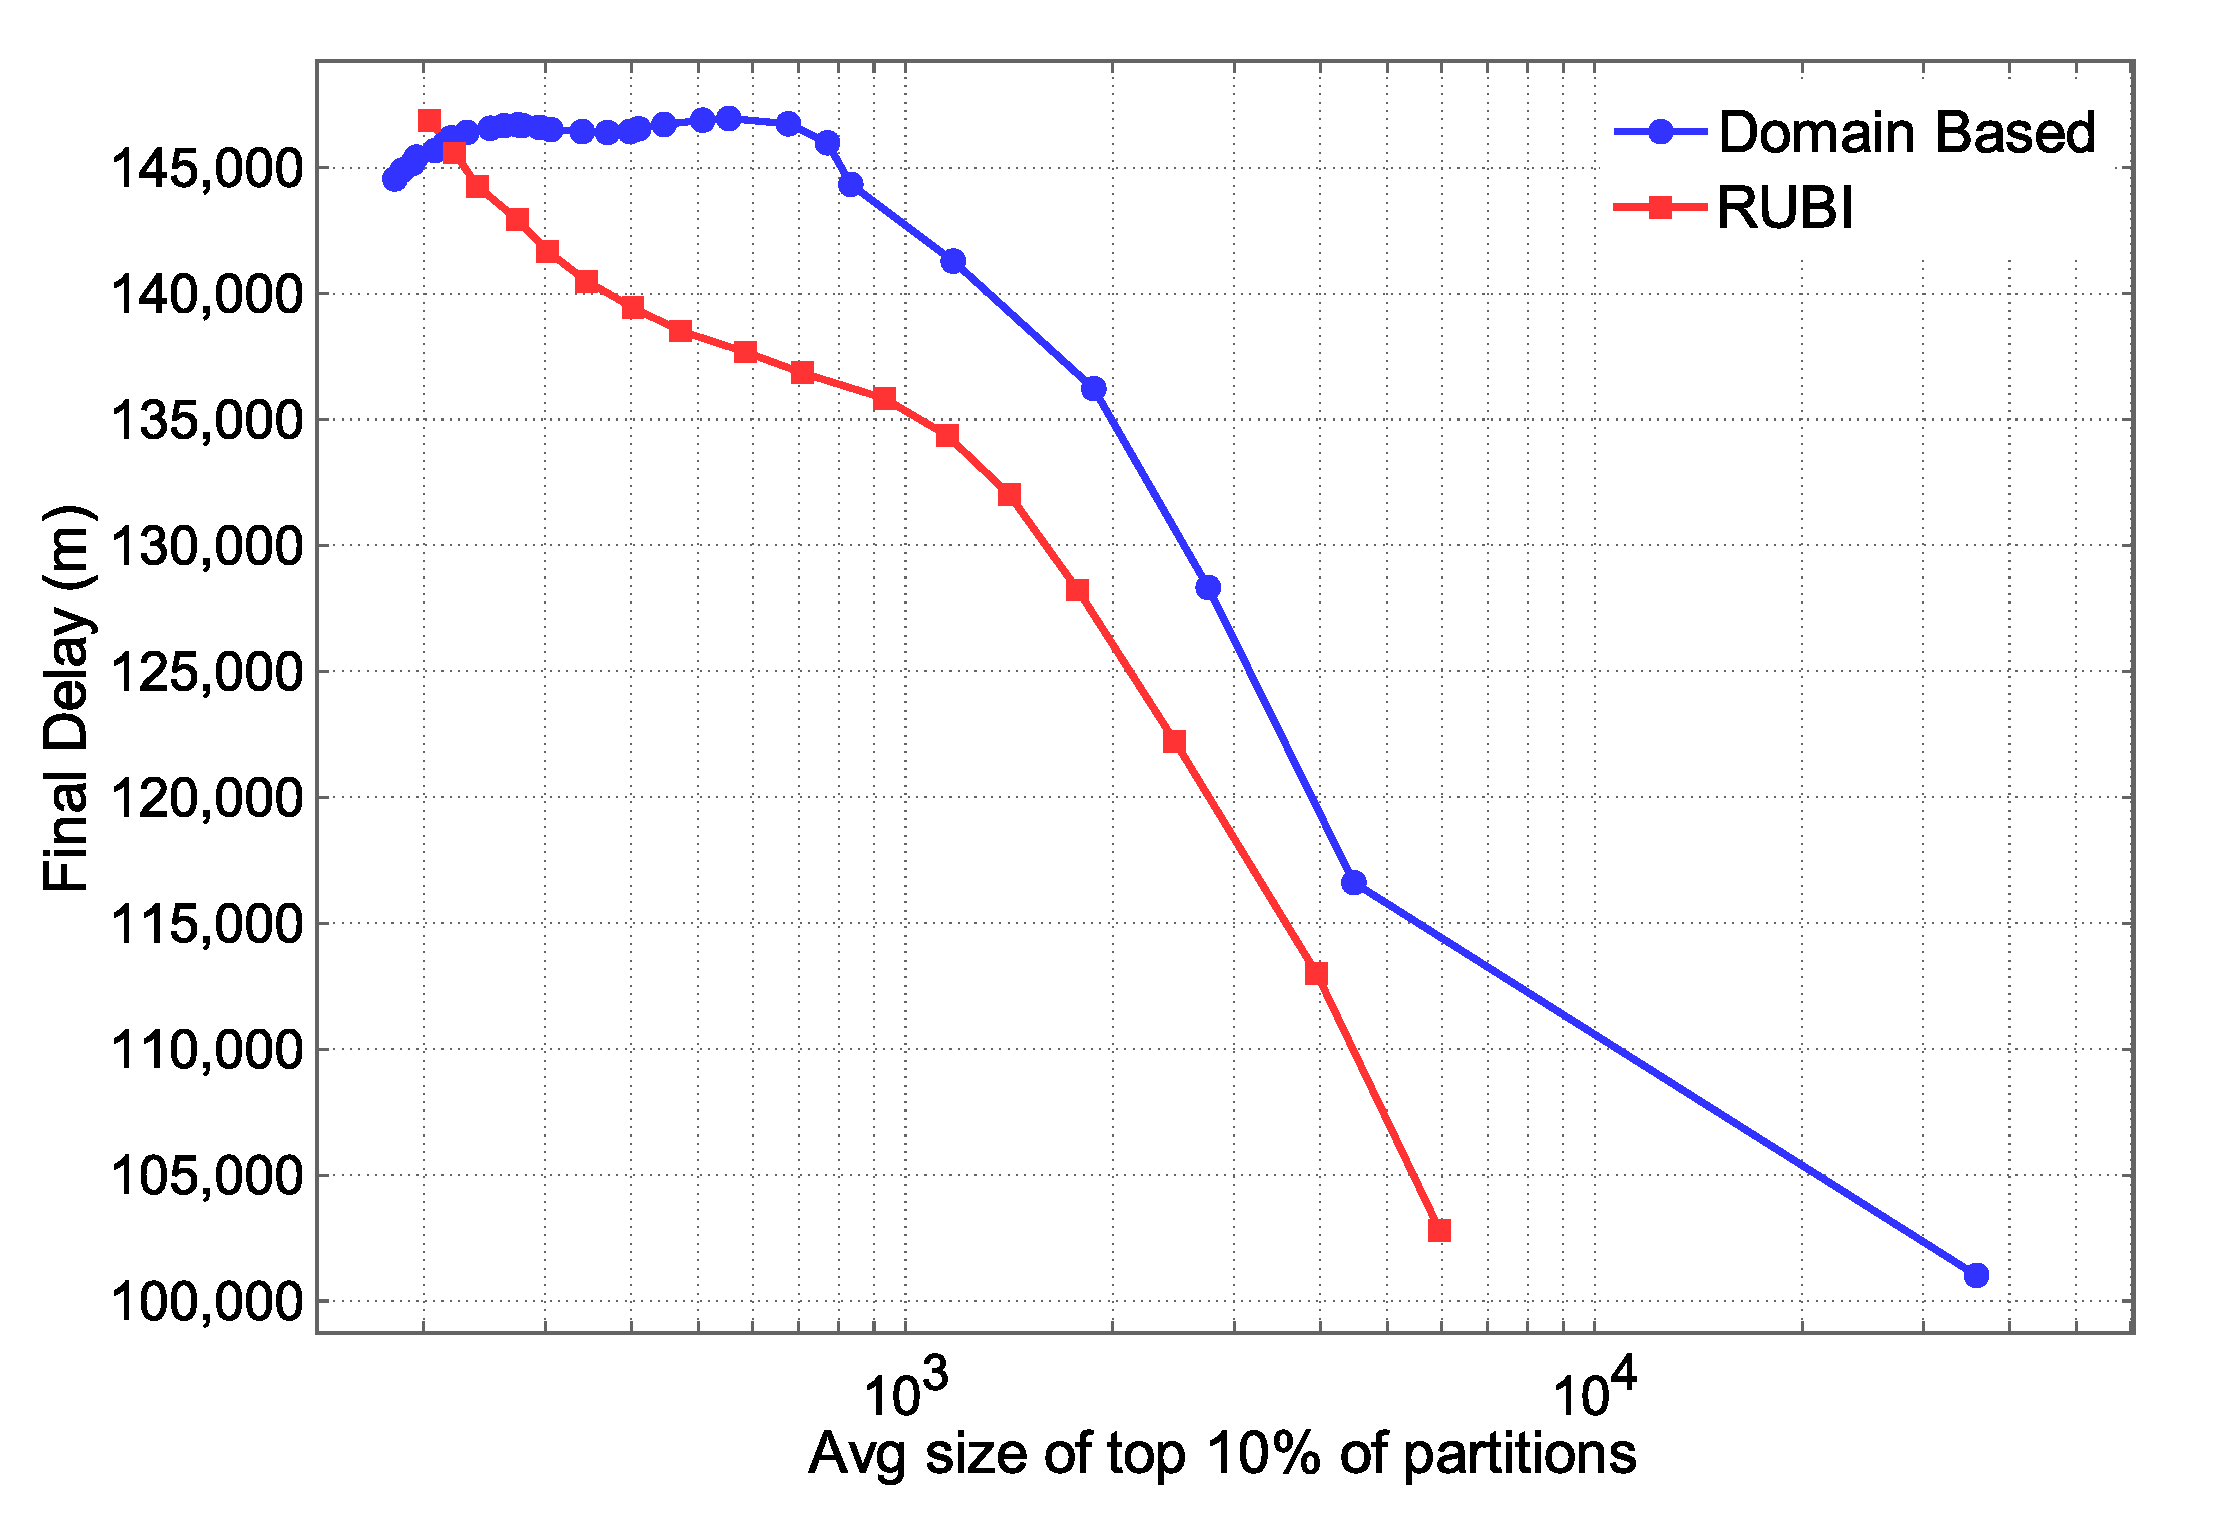
\includegraphics[width=1.0\columnwidth]{ATFMPPerformancevsAvgSize}
\caption{When comparing individual partition size averages to performance, RUBI partitions perform much better than domain specific partitions with respect to average partition size and final performance.}
\label{ATFMPPerformancevsAvgSize}
\end{figure}

\chapter{Conclusion}
The contributions of this paper are to present a distributed adaptive air traffic flow management algorithm with implementable results, and to introduce the Reward/Utility Based Impact algorithm. 

The ATFMP method introduced is based on agents representing airport gates within the NAS choosing aircraft ground delay with the intent of minimizing delay within the system. It uses reinforcement learning in combination with the difference reward and hard constraints on congestion. This is typically an impossible problem, but we introduce agent partitions to dramatically reduce the time complexity by  450x per simulation step with a 37\% increase in performance over the greedy solution. The different sizes of partitions also allowed the implementation to vary with the situation. If results need to be computed quickly, a large number of partitions could be used, where a smaller number of partitions could be used if performance was more important than speed. In this case a solution could reduce the time complexity by 5400x per learning step, with a 20\% increase in performance over the greedy solution. The ease of adding simple ground delays in combination with the large increase in performance over currently used approaches makes this approach easily deployable and effective.

%An extension of this work could be allowing agents to choose a different ground delay whenever they land for a lay over, turning the problem heterogeneous.

%Reward approx future work.
This paper also introduces RUBI, a partitioning algorithm that computes reward-based impacts that can then be used to partition agents together, removing the need for prior knowledge of the system. This method also removes the need develop similarity metrics derived from expert domain knowledge. Additionally, by removing all knowledge about the domain and partitioning based on reward, RUBI can be used to discover non-trivial indirect interactions encoded in a reward signal. Since RUBI uses only a reward signal to compute impacts, it will theoretically work in any domain where partitioning is useful.

In this work, we showed that partitioning with RUBI accurately encapsulated the amount of coupling between agents, leading to a higher self-similarity metric over the domain-based partitioning, leading to faster simulation computation times. Learning using partitions developed with RUBI also found a 37\% increase in performance over the greedy solution, but with a 510x reduction in time complexity per learning step. This reduction in simulation cost was due to partitioning with RUBI leading to a larger number of smaller sized reward independent partitions.

\section{Future Work}
Future work in the ATFMP would mainly involve increasing both performance and speed. Speed could easily be improved through the use of parallel computing and optimization of the greedy scheduler. Approaches improving team based coordination such as leniency \cite{Panait} and coordination graphs \cite{Kok:2006:CMR:1248547.1248612,Coordination} could be additional ways to increase performance at the cost of speed. Further analysis will be done to attempt to add these coordination methods to this approach while minimizing the cost to speed. A more accurate environment with a higher level of complexity could be added by making each agent heterogeneous and the domain time-extended, allowing agents to choose a different ground delay whenever they land for a lay over. Additional improvements involve a more advanced and unbiased greedy scheduler.

Future work in RUBI would involve applying it to domains where coupling is very difficult to predict. We expect that RUBI would work fine in such a domain, but more exploration is needed. Performing a formal analysis of the relation between the number of iterations of RUBI and partition performance is important for future work, as we currently do not have a formal stop criteria. Approximating the impact score of each agent, rather than using a accumulation has the potential of being very informative when performing an analysis of a system. Future work in performing a simple approximation of the local reward function for each agent will greatly speed up RUBI computation time. Lastly, performing distributed clustering would be an important, yet simple extension to this work. Agents need only to compute the difference in local rewards if they come into contact with another agent, and then partition using this trimmed down similarity matrix. 

Further advances in the simulator could be easily worked into the problem. Attributes such as flight importance or unscheduled delays, such as weather or maintenance, could be easy implemented. Additionally, a level of uncertainty can be added to analyze how robust this particular solution is to unknown changes. This approach may be dynamic enough to be robust to all of these changes, and this is a subject of further research.

\bibliographystyle{plain}
\bibliography{thesis}

\end{document}
